\chapter{The quantum logic formalism}
\label{s:QuanLog}
\section{Introduction:  measurements as logic}
\index{Quantum logic}
The quantum logic formalism is another interesting, albeit more abstract, way to formulate quantum physics.
The bonus of  this approach is that one does not have to assume that the set of observables of a physical system is embodied with the algebraic structure of an associative unital algebra. 
As we have discussed in the previous section, the fact that one can ``add'' and ``multiply'' observables is already a highly non trivial assumption.
This algebraic structure is natural in classical physics since observables form a commutative algebra, coming from the action of  adding and multiplying results of different measurements. 
In quantum physics this is not equivalent, and we have seen for instance that the GNS construction relates the algebra structure of observables to the Hilbert space structure of pure states. 
In particular to the superposition principle for states comes from the addition law for observables.
% , although a natural mathematical extension of classical mechanics. 
In the quantum logic formulations  this algebraic structure itself comes out somehow naturally from the symmetries of the measurement operations considered on the physical system.


The ``quantum logic'' approach was initiated by G. Birkhoff \footnote{An eminent mathematician, not to be confused with his father, the famous G. D. Birkhoff of the ergodic theorem} and J. von Neumann (again!) in \cite{BirkVNeumann36}.
\index{von Neumann J.}
It was then (slowly) developped, notably  by physicists like G. Mackey \cite{Mackey63}, J.~M. Jauch \cite{Jauch68} and C. Piron \cite{Piron64,Piron76}, and mathematicians like Varadarajan\cite{Varadarajan1985}.
A good reference on the subject (not very recent but very valuable) is the book by E. Beltrametti and G. Cassinelli \cite{BeltCassi81}.

The terminology ``quantum logic'' for this approach is historical and is perhaps  not fully adequate, since it does not mean that a new kind of logic is necessary to understand quantum physics. It is in fact not a ``logic'' in the mathematical sense, and it relies on the standard logics used in mathematics and exact sciences. It could rather be called ``quantum propositional calculus'' or ``quantum propositional geometry'', where the term ``proposition'' is to be understood as ``test'' or ``projective measurement'' on a quantum system.
The mathematics underlying the quantum logic formalism have  applications in various areas of mathematics, logic and computer sciences. 
The quantum logic approaches do not form a unified precise and consistent framework like algebraic quantum field theory. It has several variants, most of them insisting on propositions, but some older one relying more on the concept of states (the so called convex set approaches). Some recent formulations of quantum physics related to quantum logic have some grandiose categorial formulations.

In this course  I shall give a short, partial presentation of this approach, from a personal point of view\footnote{with the usual reservation on the lecturer's qualifications}. 
I shall try to stress where the physical concepts of causality, reversibility and locality play a role, in parallel to what I tried to do for the algebraic formalism.
My main reference and source of understanding is the review by Beltrametti and Cassinelli \cite{BeltCassi81}.
%only present what I have been able to  understand.

The idea at the root of this approach goes back to J. von Neumann's book \cite{vonNeumann32,vonNeumann32G}.
It starts from the observation that the observables given by projectors, i.e. operators $\mathbf{P}$ such that $\mathbf{P}^2=\mathbf{P}=\mathbf{P}^\dagger$, correspond to propositions with YES or NO (i.e. TRUE or FALSE) outcome in a logical system. 
\index{Projection operator}
An orthogonal projector $\mathbf{P}$ onto a linear subspace $P\subset\mathcal{H}$ is indeed the operator associated to an observable that can take only the values $1$ (and always $1$ if the state $\psi\in P$ is in the subspace $P$) or $0$ (and always $0$ if the state $\psi\in P^\perp$ belongs to the orthogonal subspace to $P$).
Thus we can consider that measuring the observable $\mathbf{P}$ is equivalent to perform a test on the system, or to check the validity of a logical proposition $\textbf{p} $ on the system. 
\begin{equation}
\label{ }
\mathbf{P}\ =\ \text{orthogonal projector onto}\ P\quad \leftrightarrow\quad\text{proposition}\ \mathbf{p}
\end{equation}
If the result is $1$ the proposition \textbf{p} is found to be TRUE, and if the result is $0$ the proposition \textbf{p} is found to be FALSE.
\begin{equation}
\label{ }
\langle\psi|\mathbf{P}|\psi\rangle=1 \implies  \textbf{p}\ \text{always TRUE on}\ |\psi\rangle
\end{equation}
The projector $\mathbf{1}-\mathbf{P}$ onto the orthogonal subspace $P^\perp$ is associated to the proposition  $\textbf{not\ p}$, meaning usually that $\textbf{p}$ is false (assuming the law of excluded middle)
\begin{equation}
\label{ }
\langle\psi|\mathbf{P}|\psi\rangle=0 \implies  \textbf{p}\ \text{always FALSE on}\ |\psi\rangle
\end{equation}
so that
\begin{equation}
\label{ }
\mathbf{1-P}\ =\ \text{orthogonal projector onto}\ P^\perp\quad \leftrightarrow\quad\text{proposition}\ \mathbf{not\ p}
\end{equation}


In classical logic the negation $\textbf{not}$ is denoted in various ways
%$\textbf{not\ A}={\boldsymbol{\neg}}\mathbf{A}$ ($=A'=\bar A=\tilde A=\sim A$).
\begin{equation}
\label{ }
\textbf{not}\ \mathbf{a}\ = \ {\boldsymbol{\neg}}\mathbf{a} \ ,\ \mathbf{a}'\ ,\ \bar{\mathbf{a}}\ ,\ \tilde{\mathbf{a}}\ ,\ \sim\! \mathbf{a}
\end{equation}
I shall use the first two notations.

Now if two projectors $\mathbf{A}$ and $\mathbf{B}$ (on two subspaces $A$ and $B$) commute, they correspond to classically compatible observables $A$ and $B$ (which can be measured independently), and to a pair of propositions $\mathbf{a}$ and $\mathbf{b}$ of standard logic.
The projector $\mathbf{C}=\mathbf{AB}=\mathbf{BA}$ on the intersection of the two subspaces $C=A\cap B$ corresponds to the proposition $\mathbf{c}= ``\mathbf{a} \ \text{and}\ \mathbf{b}''=\mathbf{a}\wedge \mathbf{b}$.
Similarly the projector $\mathbf{D}$ on the linear sum of the two subspaces  $D=A+ B$ corresponds to the proposition $\mathbf{d}$=``$\mathbf{a}$ or ${\mathbf{b}}$'' =$\mathbf{a}\vee \mathbf{b}$.
\begin{equation}
\label{AandorB}
A\cap B\quad\leftrightarrow \quad\mathbf{a}\wedge\mathbf{b}=\mathbf{a\,and\,b}
\qquad,\qquad
A+ B\quad\leftrightarrow \quad\mathbf{a}\vee\mathbf{b}=\mathbf{a\,or\,b}
\end{equation}
Finally the fact that for subspaces $A\subset B$, i.e. for projectors $\mathbf{AB}=\mathbf{BA}=\mathbf{A}$, is equivalent to state that $\mathbf{a}$ implies $\mathbf{b}$
\begin{equation}
\label{AimpliesB}
A\subset B\quad\leftrightarrow\quad \mathbf{a}\implies\mathbf{b}
\end{equation}

This is easily  extended to a general (possibly infinite) set of \emph{commuting} projectors.
Such a set generates a commuting algebra of observables $\mathcal{A}$, which corresponds to the algebra of functions on some classical space $X$. 
The set of corresponding subspaces, with the operations of  linear sum, intersection and orthocomplementation ($+,\cap,\perp$), is isomorphic to a Boolean algebra of propositions with ($\vee,\wedge,\neg$), or to the algebra of characteristic functions on subsets of $X$.
\index{Boolean algebra} 
Indeed, this is just a reformulation of ``ordinary logic''\footnote{In a very loose sense, I am not discussing mathematical logic theory.} where characteristics functions  of measurable sets  (in a Borel $\sigma$-algebra over some set $X$) can be viewed as logical propositions. 
Classically all the observables of some classical system  (measurable functions over its phase space $\Omega$) can be constructed out of the classical propositions on the system (the characteristic functions of measurable subsets of $\Omega$) . 
\index{Boolean logic}

\begin{figure}[h]
\begin{center}
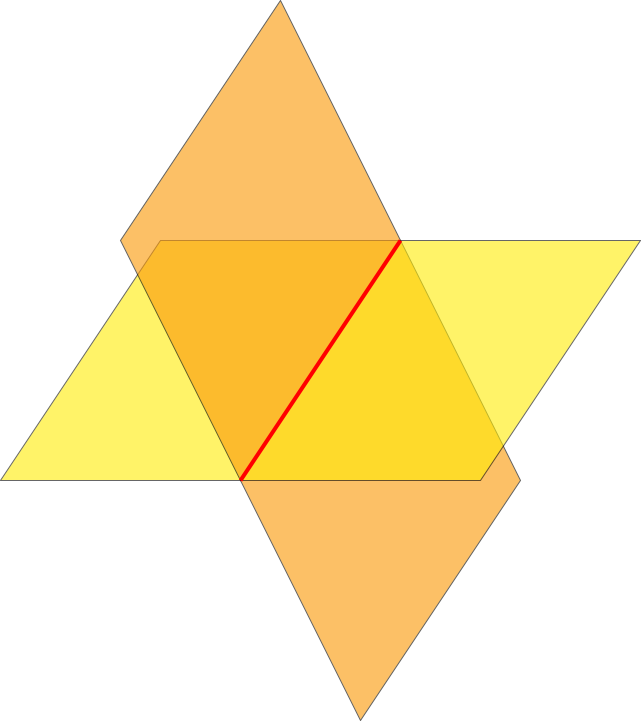
\includegraphics[width=2in]{and-planes.png}
\qquad
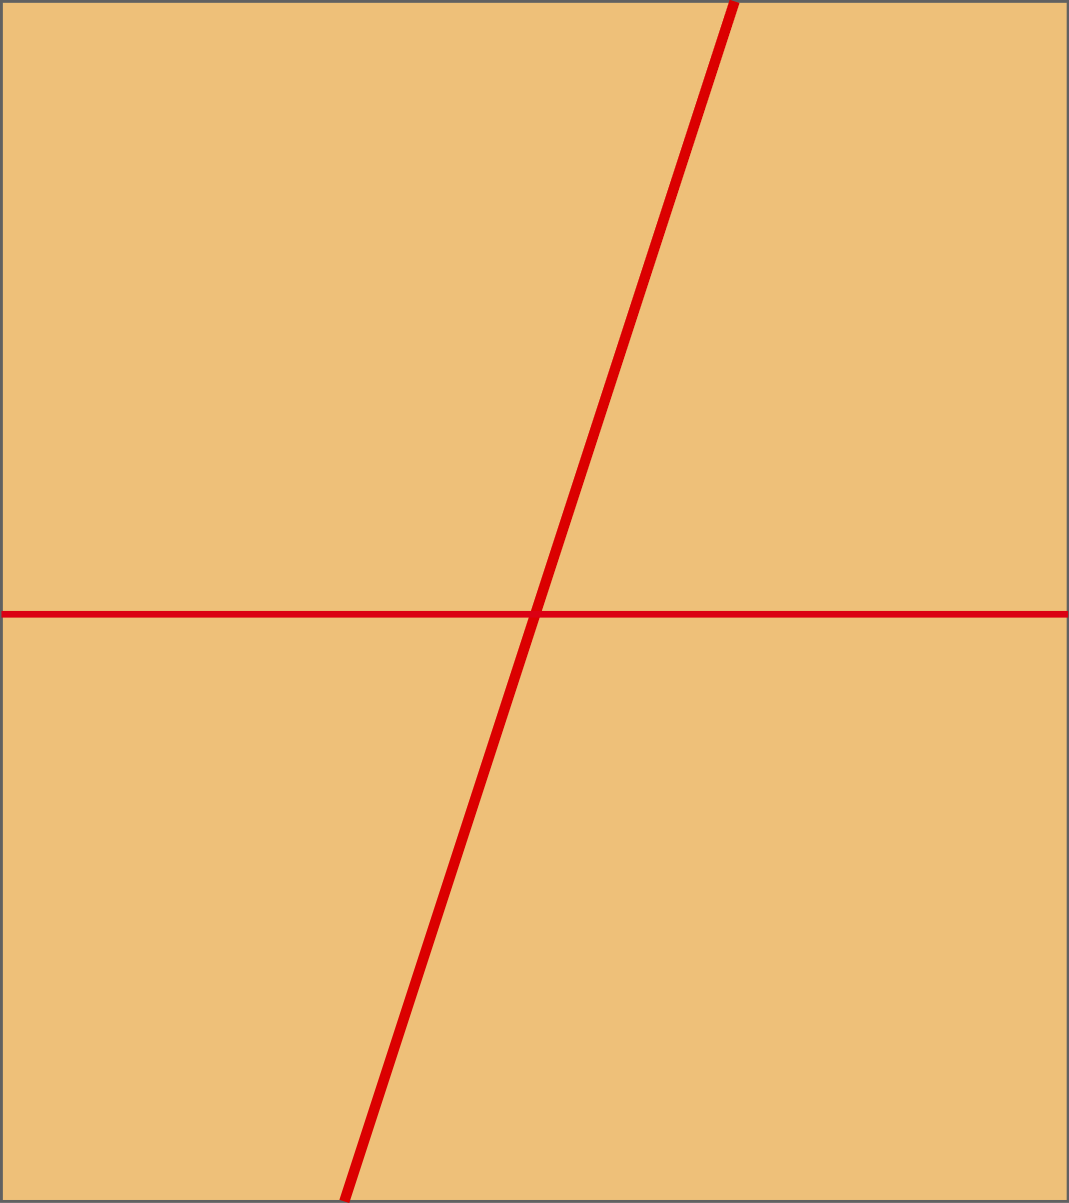
\includegraphics[width=1.5in]{or-planes.png}
\caption{The $\wedge$ as intersection and the $\vee$ as linear sum of subspaces in quantum logic }
\label{ }
\end{center}
\end{figure}


In quantum mechanics all physical observables can be constructed out of projectors. 
For general, non necessarily commuting projectors $\mathbf{A}$ and $\mathbf{B}$ on subspaces $A$ and $B$ one still associate propositions $\mathbf{a}$ and $\mathbf{b}$. The negation $\neg\mathbf{a}$, the ``and''  (or ``meet'') $\mathbf{a}\wedge\mathbf{b}$ and the ``or'' (or ``join'') $\mathbf{a}\vee\mathbf{b}$ are still defined by the geometrical operations $\perp$, $\cap$ and $+$ on subspaces given by
\ref{AandorB}. The ``implies'' $\implies$ is also defined by the $\subset$ as in \ref{AimpliesB}

However the fact that in a Hilbert space projectors do not necessarily commute implies that the standard distributivity law of propositions
\index{Distributivity}
\begin{equation}
\label{ }
A\wedge(B\vee C)=(A \wedge B)\vee(A\wedge C)\qquad\vee=\text{or}\qquad\wedge=\text{and}
\end{equation}
does not hold. It is replaced by the weaker condition ($A$, $B$, $C$ are the linear subspaces associated to the projectors $\mathbf{A}$, $\mathbf{B}$, $\mathbf{C}$)
\begin{equation}
\label{ }
%A\wedge(B\vee C)\supset(A \wedge B)\vee(A\wedge C)\qquad\vee=\text{or}=\text{union}\qquad\wedge=\text{and}=\text{intersection}
A\cap(B + C)\supset ((A \cap B)+(A\cap C))
\end{equation}
which corresponds in terms of propositions (projectors) to
\begin{equation}
\label{ }
(\mathbf{a} \wedge \mathbf{b})\vee(\mathbf{a}\wedge \mathbf{c})\implies \mathbf{a}\wedge(\mathbf{b}\vee \mathbf{c})
\end{equation}
or equivalently
\begin{equation}
\label{ }
\mathbf{a}\vee(\mathbf{b}\wedge \mathbf{c})
\implies 
(\mathbf{a} \vee \mathbf{b})\wedge(\mathbf{a}\vee \mathbf{c})
\end{equation}

A simple example is depicted on fig.~\ref{nondistplane}. The vector space $V$ in the plane (dim=2) and the subspaces $A$, $B$ and $C$ are three different coplanar lines (dim=1). $B+C=V$, hence $A\cap(B+C)=A\cap V=A$, while $A\cap B=A\cap C =\{0\}$; hence $A\cap B+A\cap C =\{0\}$.

\begin{figure}[h]
\begin{center}
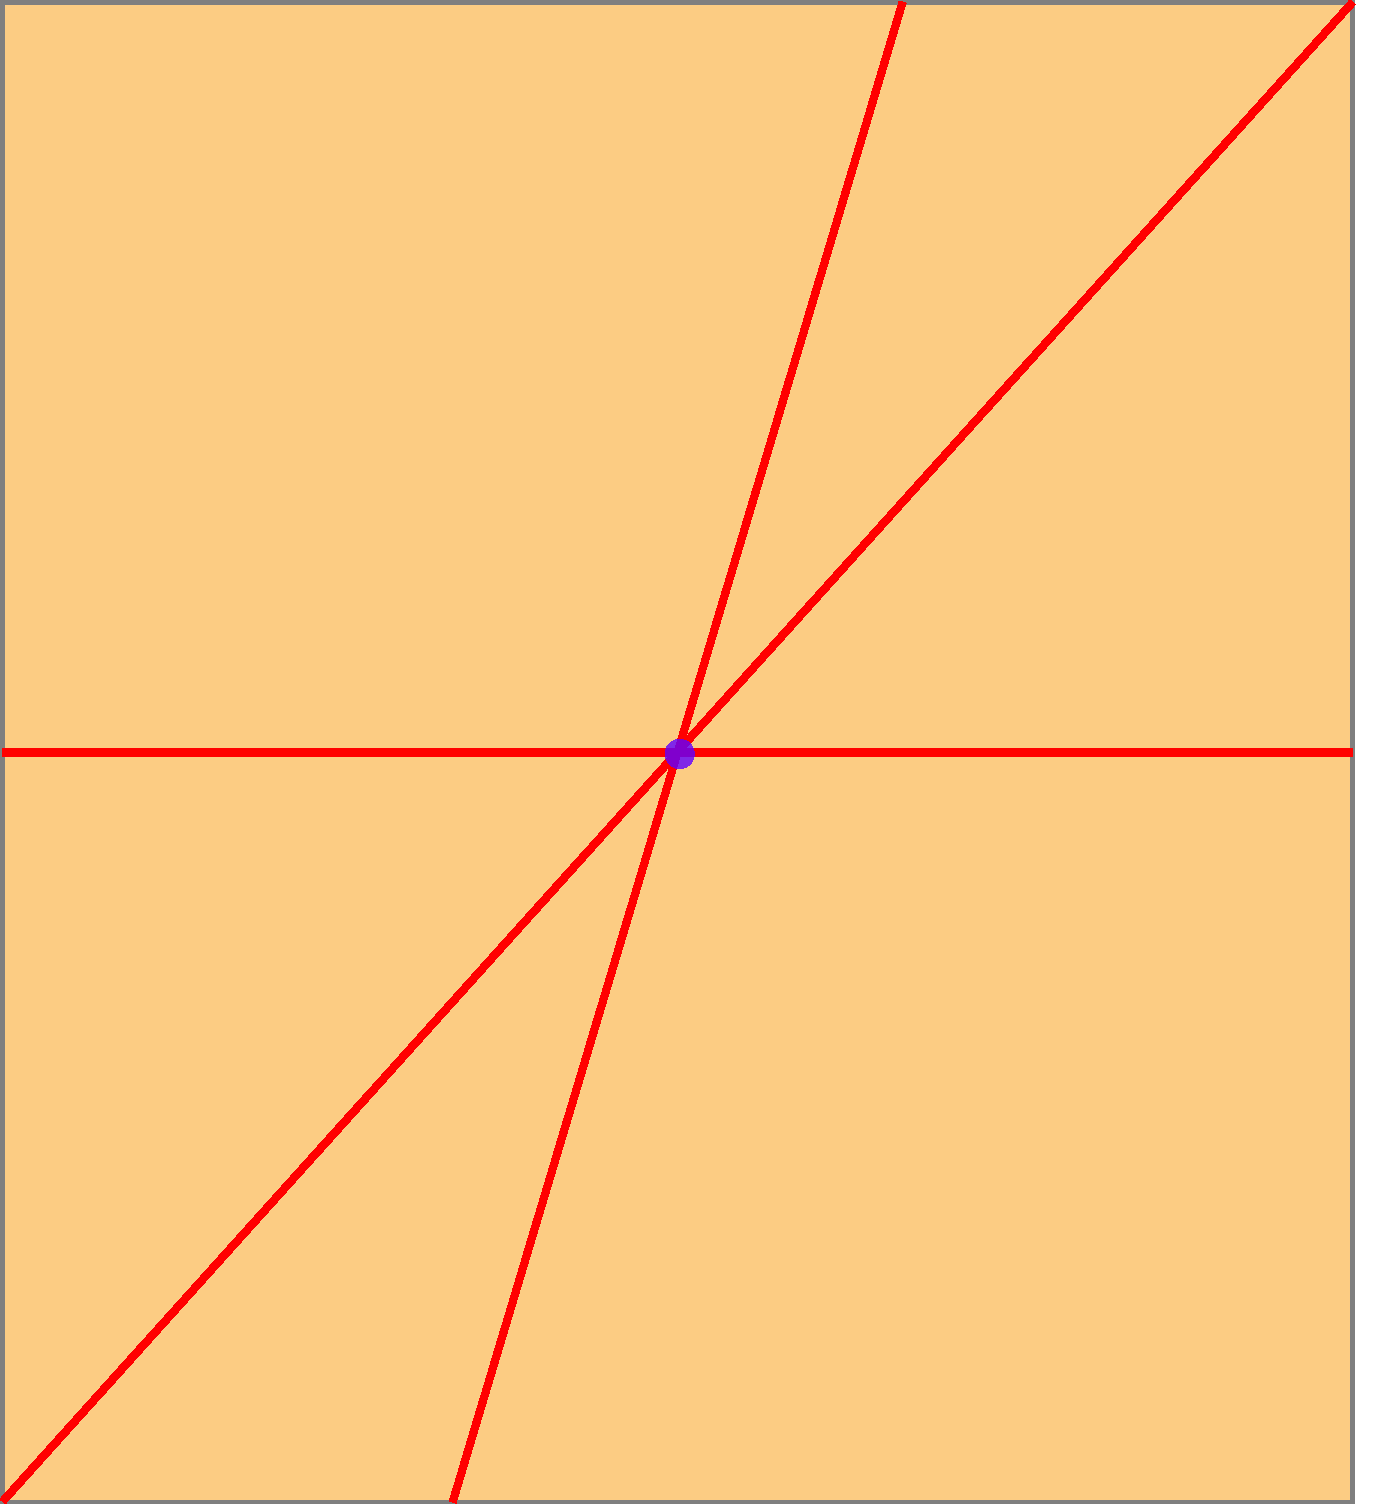
\includegraphics[width=2in]{non-distrib-planes.pdf}
\caption{A simple example of non-distributivity}
\label{nondistplane}
\end{center}
\end{figure}

Therefore the set of projectors on a Hilbert space do not generate a Boolean algebra. 
The purpose of the quantum logic approach is to try to understand what are the minimal set of consistency requirements on such propositions/measurements, based on logical consistency (assuming that internal consistency has something to do with the physical world), and on physical requirements (in particular causality, reversibility and locality) and what are the consequences for the formulation of physical laws.
I discuss the conservative approach where one does not try to use a non-classical logic (whatever it means) but discuss in a classical logic framework the statements which can be made on quantum systems.

There are many variants of the formalism: some insist on the concept and the properties of the propositions (the test), some others on those of the states (the probabilities). They are often equivalent.
Here I present a version based primarily on the propositions.

\section{A presentation of the principles}

\subsection{Projective measurements as propositions}

\index{Ideal measurement}
As explained above, in the standard formulation of quantum mechanics, projectors are associated to ``ideal'' projective measurements  (``projective measurement ``of the first kind'', or ``non-demolition'' projective measurements). The fundamental property of such measurements is that if the system is already in an eigenstate of the projector, for instance $\mathbf{P}|\psi\rangle=|\psi\rangle$, then after  measurement  the state of the system is unchanged. This means that successive measurements of $P$ give always the same result ($1$ or $\TRUE$).
Without going into  a discussion of measurements in quantum physics, let me stress that this is of course an idealisation of actual measurements. In general physical measurements are not ideal measurements, they may change the state of the system, while gaining some information on the system we in general loose some other information, they may and in general do destroy part or the whole of the system studied. Such general processes may be described by the formalism of POVM's (Projective Operator Valued Measures).

In the following presentation, I assume that such ideal repeatable measurements are (in principle ) possible for all the observable properties of a quantum system. The formalism here tries to guess what is a natural and minimal set of physically reasonable and logically consistent axioms for such measurements.

\subsection{Causality, POSET's and the lattice of propositions}
One starts from a set of propositions or tests $\mathcal{L}$ (associated to ideal measurements of the first kind on a physical system)
%non demolition yes-no measurements on a physical system) 
and from a set of states $\mathcal{E}$ (in a similar sense as in the algebraic formulation, to be made more precise along the discussion).
On a given state $\varphi$ the test (measurement) of the proposition $a$ can give TRUE (i.e. YES or $1$) or FALSE (NO or $0$).
It gives TRUE with some probability. In this case one has extracted information on the system, which is now (considered to be) in a state $\varphi_a$.


I note $\varphi(a)$
%$=P_\phi(a)=E_\phi[a\to\TRUE]$ = 
the probability that $a$ is found $\TRUE$, assuming that the system was in state $\varphi$ before the test.
I shall not discuss at that stage what I mean exactly by probability (see the previous discussions).
\\

\subsubsection{Causal order relation:}
The first ingredient is to assume that there an order relation $a\preceq b$ between propositions. Here it will be defined by the causal relation
\begin{equation}
\label{preceqdef}
a\preceq b\quad\iff\quad\text{for any state $\phi$, if $a$ is found true, then $b$ will be found true}
\end{equation}
Note that this definition is  causal (or dynamical) from the start, as to be expected in quantum physics.
It is equivalent to 
\begin{equation}
\label{preceqstate}
a\preceq b\quad\iff\quad\forall\ \phi\ ,\ \ \phi_a(b)=1
\end{equation}

One assumes that this causal relation has the usual properties of a partial order relation.
This amounts to enforce relations between states and propostions.
First one must have:
\begin{equation}
\label{aperceqa}
a\preceq a
\end{equation}
This means that if $a$ has been found true, the system is now in a state such that $a$ will always be found true.
Second one assumes also that
\begin{equation}
\label{preceqeq}
a\preceq b\ \text{and}\ b\preceq c\ \implies \ a\preceq c
\end{equation}
This is true in particular when, if the system is in a state $\psi$ such that $b$ is always true, then after measuring $b$, the system is still is the same state $\psi$. In other word, $\psi(b)=1\implies \psi_b=\psi$. This is the concept of repeatability discussed above.

These two properties makes $\preceq$ a \emph{preorder relation}.
\index{Preorder relation}

One also assumes that
\begin{equation}
\label{precprec}
a\preceq b\ \text{and}\ b\preceq a\quad \implies \quad a=b
\end{equation}
This means that tests which give the same results on any states are indistinguishable.
This also means that one can identify a proposition $a$ with the set of states such that $a$ is always found to be true (i.e. $\psi(a)=1$).
\ref{precprec} makes $\preceq$ a partial order relation and $\mathcal{L}$ a \emph{partially ordered set} or POSET.
\index{POSET}

%\paragraph{AND (or meet):}
\subsubsection{AND (meet $\wedge$):}
The second ingredient is the notion of logical cunjunction AND.
One assumes that for any pair of test $a$ and $b$, there is a \emph{unique greater proposition} $a\wedge b$ such that
\begin{equation}
\label{andcunj}
a\wedge b\preceq a \ \text{and}\ \ a\wedge b\preceq b
\end{equation}
in other word, there is a unique $a\wedge b$ such that
$$c\preceq a\ \text{and}\  c\preceq b \ \ \implies\ \ c\preceq a\wedge b$$
NB: this is a non trivial assumption, not a simple consequence of the previous ones. 
It can be justified  using the notion of filters (see Jauch) or that of questions associated to propositions (see Piron).
Here to make things simpler I just present it as an assumption. 
On the other hand it is very difficult to build anything without this assumption.
Note that \ref{andcunj} implies \ref{precprec}.

This definition extends to any set $\mathcal{A}$ of propositions 
%$\bigwedge_{\mathcal A}$
\begin{equation}
\label{ }
\bigwedge{\mathcal A}=\mathop{\bigwedge}\{{a\in\mathcal{A}}\}=\text{greatest}\ c:\ c\preceq a,\ \forall a\in\mathcal{A}
\end{equation}
%$$\bigwedge{\mathcal A}=\mathop{\bigwedge}\{{a\in\mathcal{A}}\}=\text{greatest}\ c:\ c\preceq a,\ \forall a\in\mathcal{A}$$
I do not discuss if the set $\mathcal{A}$ is finite or countable.

%\paragraph{Logical OR (or join):}
\subsubsection{Logical OR (join $\vee$):}

From this we can infer the existence of a logical OR (by using Birkhoff theorem)
\begin{equation}
\label{ }
a\vee b=\bigwedge\{c\,:\ a\preceq c\ \text{and}\ b\preceq c\}
\end{equation}
which extents to sets of propositions
\begin{equation}
\label{ }
\bigvee\mathcal{A}=\bigwedge\{b\,:\ a\preceq b\ ,\ \forall a\in\mathcal{A}\}
\end{equation}

%\paragraph{Trivial $\mathbf{1}$ and vacuous $\emptyset$ propositions:}
\subsubsection{Trivial $\mathbf{1}$ and vacuous $\emptyset$ propositions:}

It is natural to assume that there is a proposition $\mathbf{1}$ that is always true 
\begin{equation}
\label{ }
\text{for any state $\phi$,  $\mathbf{1}$ is always found to be true, i.e. $\phi(\mathbf{1})=1$}
\end{equation}
and another proposition $\emptyset$ that is never true
\begin{equation}
\label{ }
\text{for any state $\phi$,  $\emptyset$ is never found to be true, i.e. $\phi(\emptyset)=0$}
\end{equation}
Naturally one has
\begin{equation}
\label{ }
\mathbf{1}=\bigvee\mathcal{L}\ \text{and}\ \ \emptyset=\bigwedge\mathcal{L}
\end{equation}
With these assumptions and definitions the set of propositions $\mathcal{L}$  has now the structure of a  \textbf{complete lattice}.
%forms a partially ordered set or POSET, with the structure of a  \textbf{complete lattice}.
\index{Complete lattice}

\subsection{Reversibility and  orthocomplementation}

\subsubsection{Negations $\mathbf{a}'$ and $'\mathbf{a}$}
I have not yet discussed what to do if a proposition is found to be false.
To do so one must introduce the seemingly simple notion of negation or complement.
In classical logic this is easy. The subtle point is that for quantum systems, where causality matters, there are two inequivalent ways to introduce the negation.
These two definitions becomes equivalent only if one assumes that propositions on quantum systems share a property of causal reversibility. 
In this case, one recovers the standard negation of propositions in classical logic, and ultimately this will lead to the notion of orthogonality and of scalar product of standard quantum mechanics. 
Thus here again, as in the previous section, reversibility appears to be one of the essential feature of the principles of quantum physics.
%I shall show that the logically standard properties of the negation are in fact  deeply connected to causal reversibility.

%\paragraph{Negation - d�finition 1 (or complement proposition):}
\paragraph{Negation - d�finition 1:}

To any proposition $a$ one can associate its negation (or complement proposition) $a'$ defined as
\begin{equation}
\label{ }
\text{for any state $\phi$, if $a$ is found to be true, then $a'$ will be found to be false}
\end{equation}
$a'$ can be defined equivalently as
\begin{equation}
\label{ }
a'=\bigvee\{b\,\text{such that}\ \text{on any state $\phi$, if $a$ is found true, then $b$ will be found false}\}
\end{equation}
%
%\par\noindent{$\textdbend$}\textbf{Important warning about causality and non-reversibility!}
%
\paragraph{Negation - d�finition 2:}
It is important at that stage to realize that, because of the causality ordering in the definition, there is an alternate definition for the complement,  that I denote $'\!a$, given by
\begin{equation}
\label{ }
\text{for any state $\phi$, if $'\!a$ is found to be true, then $a$ will be found to be false}
\end{equation}
or equivalently
\begin{equation}
\label{ }
'\!a=\bigvee\{b\,;\ \text{such that on any state $\phi$ , if $b$ is found  true, then $a$ will be found false}\}
\end{equation}
These two definitions are \emph{not equivalen}t, and they do not necessarily fulfill the properties of the negation in classical propositional logic
%\footnote{I do not discuss the intuitionist versus standard logics debate.}
\footnote{The point discussed here is a priori not connected to the classical versus intuitionist logics debate. Remember that we are not discussing a logical system.}
.
\begin{equation*}
\label{ }
\neg{(\neg a)}\mathop{=}a\ \ \text{and}\ \ \ \neg(a\wedge b)\mathop{=}  \neg a\vee \neg b
%\qquad\text{\textbf{are not necessarily true!}}
\end{equation*}
These problems come from the fact that the definition for the causal order $a\preceq b$ does not implies that $b'\preceq a'$, as in classical logic. Indeed  the definition \ref{preceqdef} for $a\preceq b$ implies that for every state
\begin{equation}
\label{ }
\text{if $b$ is found false, then $a$ was found false}
\end{equation}
while $b'\preceq a'$ would  mean
%we expect that for a well behaved negation, $b'\preceq a'$, which  means
\begin{equation}
\label{ }
\text{if $b$ is found false, then $a$ will be found false}
\end{equation}
or equivalently
\begin{equation}
\label{ }
\text{if $a$ is found true, then $b$ was found true}
\end{equation}

%\subsubsection{Causal reversibility and negation$\mathbf{\neg a}$}
\subsubsection{Causal reversibility and negation}

In order to build a formalism consistent with what we know of quantum physics, we need to enforce the condition that the causal order structure on propositions is in fact independent of the choice of a causal arrow \og if $\cdots$, then $\cdots$ will $\cdots$ \fg{} versus \og if $\cdots$, then $\cdots$ was $\cdots$ \fg{} . This is nothing but the requirement of causal reversibility and it is enforced by the following simple but very important condition.
\index{Negation}
\index{Reversibility}

\paragraph{Causal reversibility:}
One assumes that the negation $a'$ is such that
\begin{equation}
\label{negrev}
a\preceq b\quad\iff\quad b'\preceq a'
\end{equation}

With this assumption, it is easy to show that the usual properties of  negation are satisfied. 
The two alternate definitions of negation are now equivalent
\begin{equation}
\label{ }
a'={'}a=\neg a
\end{equation}
and may be denoted by the standard logical symbol $\neg$.
We then have
\begin{equation}
\label{aprimeprime}
{(a')}'=a
\end{equation}
and
\begin{equation}
\label{awedgebprime}
(a\wedge b)'=a'\vee b'\
\end{equation}
as well as
\begin{equation}
\label{zerooneprime}
\emptyset=\mathbf{1}'\ ,\ \ \emptyset'=\mathbf{1}
\end{equation}
and
\begin{equation}
\label{aaprime}
a\wedge a'=\boldsymbol{\emptyset}
\ ,\ \ 
a\vee a'=\mathbf{1}
\end{equation}

A lattice $\mathcal{L}$ with a complement with the properties \ref{negrev}-\ref{aaprime} is called an \emph{orthocomplemented complete lattice} (in short OC lattice).
For such a lattice, the couple $(a,a')$ describes what is called a perfect measurement.
\index{Orthocomplementation}

\paragraph{NB:} Note that in Boolean logic, the implication $\to$ can be defined from the negation $\lnot$. Indeed  $a\to b$ means $\neg a\lor b$. Here it is the negation $\neg$ which is defined out of the implication $\preceq$.


\subsubsection{Orthogonality}
%\paragraph{Orthogonal propositions:}
With reversibility and complement, the set of propositions starts to have properties similar to the set of projections on  linear subspaces of a Hilbert space%
\footnote{One should be careful for infinite dimensional Hilbert spaces and general operator algebras. Projectors correspond in general to orthogonal projections on closed subspaces.}. 
The complement $a'$ of a proposition $a$ is similar to the orthogonal subspace $P^\perp$ of a subspace $P$.
%\textit{Can we consider $a$ and $a'$ as perfect measurements?}
This analogy can be extended to the general concept of orthogonality.

%\textbf{Definition:}
%orthogonal propositions. 
%Two proposition $a$ and $b$ are orthogonal, and noted $a\perp b$, if $b\preceq a'$ (or equivalently $a\preceq b'$).
\paragraph{Orthogonal propositions:}
\begin{equation}
\label{ }
\text{Two proposition $a$ and $b$ are orthogonal,  if $b\preceq a'$ (or equivalently $a\preceq b'$).}
\end{equation}
This is noted
\begin{equation}
\label{ }
a\perp b
\end{equation}

\paragraph{Compatible propositions:}\ \\
OC lattices contain also the concept of classical propositions. 
A subset of an OC lattice $\mathcal{L}$ is a sublattice $\mathcal{L}'$ if it is  stable under the operations $\wedge$, $\vee$ and $'$ (hence it is itself   an OC lattice). 
To any subset $\mathcal{S}\subset\mathcal{L}$ on can associate the sublattice $\mathcal{L}_\mathcal{S}$ generated by $\mathcal{S}$, defined as the smallest sublattice $\mathcal{L}'$ of $\mathcal{L}$ which contains $\mathcal{S}$.

A (sub)lattice is said to be \emph{Boolean} if it satisfy the distributive law of classical logic $a\wedge(b\vee c)=(a\wedge b)\vee(a\wedge  c)$.

A subset $\mathcal{S}$ of an OC lattice is said to be a subset of \emph{compatible propositions} if the generated lattice $\mathcal{L}_\mathcal{S}$ is Boolean.

Compatible propositions are the analog of commuting projectors, i.e. compatible or commuting observables in standard quantum mechanics.
For a set of compatible propositions, one expects that the expectations of the outcomes YES or NO will satisfy the rules of ordinary logic.



\paragraph{Orthogonal projection:}
\index{Orthogonal projector}
The notion of orthogonal projection onto a subspace can be also formulated in this framework as
\begin{equation}
\label{ }
\text{projection of $a$ onto $b$ $=\Phi_b(a)=b\wedge (a\vee b')$}
\end{equation}
This projection operation is often called the Sasaki projection. Its dual $(\Phi_b(a'))'=b'\vee(a\wedge b)$ is called the Sasaki hook $(b\mathop{\to}\limits^S a)$.
It has the property that even if $a\npreceq b$, if for a state $\psi$ the Sasaki hook  $(a\mathop{\to}\limits^S b)$ is always true, then for this state $\psi$, if $a$ is found true then $b$ will always  be  found true.
\index{Sasaki projection}
\index{Sasaki hook}


%A lattice $\mathcal{L}$ with a complement with the properties \ref{negrev}-\ref{aaprime} is called an orthocomplemented complete lattice.


\subsection{Subsystems of propositions and orthomodularity}

\subsubsection{What must replace distributivity?}

The concept of orthocomplemented lattice of propositions is not sufficient to reconstruct a consistent quantum formalism.
There are mathematical reasons and physical reasons.

One reason is that if the distributive law $A\land((B\lor C)=(A\land B)\lor(A\land C)$ is known not to apply, assuming no restricted distributivity condition is not enough and leads to too many possible structures.
In particular in general a lattice with an orthocomplementation $\neg$ may be endowed with several inequivalent ones! 
This is  problematic for the physical interpretation of the complement as $a\to\TRUE\ \iff\ a'\to\FALSE$.
\index{Distributivity}

Another problem is that in physics one is led to consider conditional states and conditional  propositions. 
In classical physics this would correspond to the restriction to some  subset  $\Omega'$ of the whole phase space $\Omega$ of a physical system, or to the projection $\Omega\to\Omega'$.
Such projections or restrictions are necessary if there are some constraints on the states of the system, if one has access only to some subset of all the physical observables of the system, or if one is interested only in the study of a subsystem of a larger system.
%that caracterize  the degrees of freedom of the system we are interested in, for instance because they correspond to the physical quantities we can measure.
In particular such a separation of the degrees of freedom is  very important when discussing locality: we are interested in the properties of the system we can associate to (the observables measured in) a given interval of space and time, as already discussed for algebraic QFT.
It is also very important when discussing effective low energy theories: we want to separate (project out) the (un-observable) high energy degrees of freedom from the (observable) low energy degrees of freedom.
And of course this is crucial to discuss open quantum systems, quantum measurement processes, decoherence processes, and the emergence of classical degrees of freedom and classical behaviors in quantum systems.

\subsubsection{Sublattices and weak-modularity}
\index{Weak modularity}
In general a subsystem is defined from the observables (propositions) on the system which satisfy some constraints.
One can reduce the discussion to one constraint $a$.
If $\mathcal{L}$ is an orthocomplemented lattice and $a$ a proposition of  $\mathcal{L}$, let us considers the subset $\mathcal{L}_{<a}$ of all propositions which imply $a$
\begin{equation}
\label{Linfadef}
\mathcal{L}_{<a}=\{b\in\mathcal{L}: \ b\preceq a\}
\end{equation}
One may also consider the subset of propositions $\mathcal{L}_{>a}$ of propositions implied by $a$
\begin{equation}
\label{Lsupadef}
\mathcal{L}_{>a}=\{b\in\mathcal{L}: \ a\preceq b\}=\left(\mathcal{L}_{<a'}\right)'
\end{equation}
The question is: is this set of propositions $\mathcal{L}_{<a}$  still an orthocomplemented lattice? One takes as order relation $\preceq$, $\vee$ and $\wedge$ in $\mathcal{L}_{<a}$ the same than in $\mathcal{L}$ and as trivial and empty propositions $\mathbf{1}_{<a}=a$, $\emptyset_{<a}=\emptyset$. 
Now, given a proposition $b\in\mathcal{L}_{<a}$, one must define what is its complement  $b'_{\scriptscriptstyle{<a}}$ in $\mathcal{L}_{<a}$. A natural choice is 
\begin{equation}
\label{ }
b'_{\scriptscriptstyle{<a}}=b'\wedge a
\end{equation}
but in general with such a choice  $\mathcal{L}_{<a}$ is not an orthocomplemented lattice, since it is easy to find for general AC lattices counterexamples such that one may have 
$b\vee b'_{\scriptscriptstyle{<a}}\neq a$. 

\paragraph{Weak-modularity:}
In order for  $\mathcal{L}_{<a}$ to be an  orthocomplemented lattice  (for any $a\in\mathcal{L}$), the orthocomplemented lattice $\mathcal{L}$ must satisfy the weak-modularity condition
\begin{equation}
\label{ }
b\preceq a\ \  \implies\ \ (a\wedge b')\vee b=a
\end{equation}
This condition is also sufficient.

\subsubsection{Orthomodular lattices}
\index{Orthomodular lattice}
\paragraph{Orthomodularity:}
An OC lattice which satisfies the weak-modularity condition is said to be an \emph{orthomodular lattice} (or OM lattice)\footnote{In French: treillis orthomodulaire, in German: Orthomodulare Verband.}. 
Clearly if $\mathcal{L}$ is OM, for any $a\in\mathcal{L}$, $\mathcal{L}_{<a}$ is also OM, as well as $\mathcal{L}_{>a}$.



\paragraph{Equivalent definitions:}
Weak-modularity has several equivalent definitions. 
Here are two interesting ones:
\begin{itemize}
  \item $a\preceq b\ \implies\ a\ \text{and}\ b\ \text{are compatible}.$
  \item the orthocomplementation  $a\to a'$ is unique in $\mathcal{L}$. 
\end{itemize}

\paragraph{Irreducibility:}
For such lattices one can also define the concept of irreducibility.
We have seen that two elements $a$ and $b$ of $\mathcal{L}$ are compatible (or commute) if they generate a Boolean lattice. The center  $\mathcal{C}$ of a lattice $\mathcal{L}$ is  the set of $a\in\mathcal{L}$ which commute with all the elements of the lattice $\mathcal{L}$. It is obviously a Boolean lattice.
A lattice is irrreducible if its center $\mathcal{C}$ is reduced to the trivial lattice $\mathcal{C}=\{\emptyset,\mathbf{1}\}$.
\index{Irreducible lattice}

\subsubsection{Weak-modularity versus modularity}
\paragraph{NB:} The (somewhat awkward) denomination \og weak-modularity\fg{} is historical. 
Following Birkhoff and von Neumann the stronger  \og modularity\fg{} condition for lattices was first considered.
\index{Modularity}
Modularity is defined as
\begin{equation}
\label{ }
a\preceq b \ \implies\ (a\lor c)\land b=a\lor(c\land b)
\end{equation}
Modularity is equivalent to weak modularity for finite depth lattices (as a particular case the set of projectors on a finite dimensional Hilbert space for a modular lattice).
But modularity turned out to be inadequate for infinite depth lattices (corresponding to the general theory of projectors in infinite dimensional Hilbert spaces).
The theory of modular lattice has links with some  W$^*$-algebras and the theory of ``continuous geometries'' (see e.g. \cite{Von-Neumann:1960fk}).


\subsection{Pure states and AC properties}
Orthomodular (OM) lattices are a good starting point to consider the  constraints that we expect for the set of ideal measurements on a physical system, and therefore to study how one can represent its states. 
In fact one still needs two more assumptions, which seem technical, but which are also very important (and quite natural from the point of view of quantum information theory). They rely on the concept of atoms, or minimal proposition, which are the analog for propositions of the concept of minimal projectors on of pure states in the algebraic formalism.

\subsubsection{Atoms}
An element $a$ of an OM lattice is said to be  an atom if
\index{Atom}
\begin{equation}
\label{ }
b\preceq a\quad\text{and}\quad b\neq a\quad\implies\quad b=\emptyset
\end{equation}
This means that $a$ is a minimal non empty proposition; it is not possible to find another proposition compatible with $a$ which allows to obtain more information on the system than the information obtained if $a$ is found to be TRUE. 

Atoms are the analog of projectors on pure states in the standard quantum formalism (pure propositions). Indeed, if the system in in some state $\psi$, before the measurement of $a$, if $a$ is an atom and is found to be true, the system will be in a pure state $\psi_a$ after the measure.

\subsubsection{Atomic lattices}
\index{Atomic lattice}
A  lattice is said to be atomic if any non trivial proposition $b\neq\emptyset$ in $\mathcal{L}$ is such that there is at least one atom $a$ such that $a\preceq b$ (i.e. any proposition \og contains\fg{} at least one minimal non empty proposition). For an atomic OM lattice one can show that any proposition $b$ is then the union of its atoms (atomisticity).

\subsubsection{Covering property}
\index{Covering property}
Finally one needs also the covering property. The formulation useful in the quantum framework is to state that if $a$ is a proposition and $b$ an atom not in the complement $a'$ of $a$, then the Sasaki projection of $b$ onto $a$, $\Phi_a(b)=a\wedge(b \vee a')$, is still an atom. 

The original definition of the covering property for atomic lattices by Birkhoff is: for any $b\in\mathcal{L}$ and any atom $a\in\mathcal{L}$ such that $a\wedge b=\emptyset$, $a\vee b$ covers $b$, i.e. there is no $c$ between $b$ and $a\vee b$ such that $b\prec c\prec a\vee b$.

This covering property is very important. It means that when reducing a system to a subsystem by some constraint (projection onto $a$), one cannot get a non-minimal proposition out of a minimal one. 
This would mean that one could get more information out of a subsystem than from the greater system.
In  other word, if a system is in a pure state, performing a perfect measurement can only map it onto another pure state. Perfect measurements cannot decrease the information on the system.

%The covering property is in fact also related to the superposition principle in the standard formulation of quantum mechanics.
\textit{The covering property is in fact also related to the superposition principle. Indeed, it implies that (for irreducible lattices) for any two difference atoms $a$ and $b$, there must be a third atom $c$ different from $a$ and $b$ such that $c\prec a\vee b$. Thus, in the weakest possible sense (remember we have no addition) $c$ is a superposition of $a$ and $b$.
CHECK}

\medskip
An atomistic lattive with the covering property is said to be an AC  lattice.
As mentionned before these properties can be formulated in term of the properties of the set of states on the lattice rather than in term of the propositions.
I shall not discuss this here.

\section{The geometry of orthomodular AC lattices}

I have given one (possible and personal) presentation of the principles at the basis of the quantum logic formalism. It took some time since I tried  to explain both the mathematical formalism and the underlying physical ideas.
I now explain the main mathematical result: the definition of the set of propositions (ideal measurements) on a quantum system as an orthomodular AC lattice can be equivalently represented as the set of orthogonal projections on some \og generalized Hilbert space \fg{}.

\subsection{Prelude: the fundamental theorem of projective geometry}
\index{Projective geometry}
The idea is to extend a classical and beautiful theorem of geometry, the Veblen-Young theorem. 
Any abstract projective geometry can be realized as the geometry of the affine subspaces of some  left-module (the analog of vector space) on a division ring $K$ (a division ring is a non-commutative field). This result is known as the \og coordinatization of projective geometry\fg{}.
Classical references on geometry are the books by E. Artin Geometric Algebra \cite{Artin:1957hs}, R. Baer \textsl{Linear algebra and projective geometry} \cite{Baer:2005kc} or Conway .
More precisely, a geometry on a linear space is simply defined by a set of points $X$, and a set of lines $\mathcal{L}$ of $X$ (simply a set of subsets of $X$). 
\index{Veblen's axiom}
\index{Veblen-Young theorem}
\index{Division ring}

\paragraph{Theorem:}
If the geometry satisfies the following axioms:
\begin{enumerate}
  \item Any line contains at least 3 points,
  \item Two points lie in a unique line,
  \item A line meeting two sides of triangle, not at a vertex of the triangle, meets the third side also (Veblen's axiom),
  \item There are at least 4 points non coplanar (a plane is defined in the usual way from lines),
  \end{enumerate}
 then the corresponding geometry is the geometry of the affine subspaces of a left module $M$ on a division ring $K$ (a division ring is a in general non-commutative field).
 
 \paragraph{Discussion:}
 The theorem here is part of the Veblen-Young theorem, that encompasses the cease when the 4th axiom is not satisfied.
The first two axioms define a line geometry structure such that lines are uniquely defined by the pairs of points, but with some superposition principle.
 The third axiom is represented on \ref{Veblen}.
 \begin{figure}[h]
\begin{center}
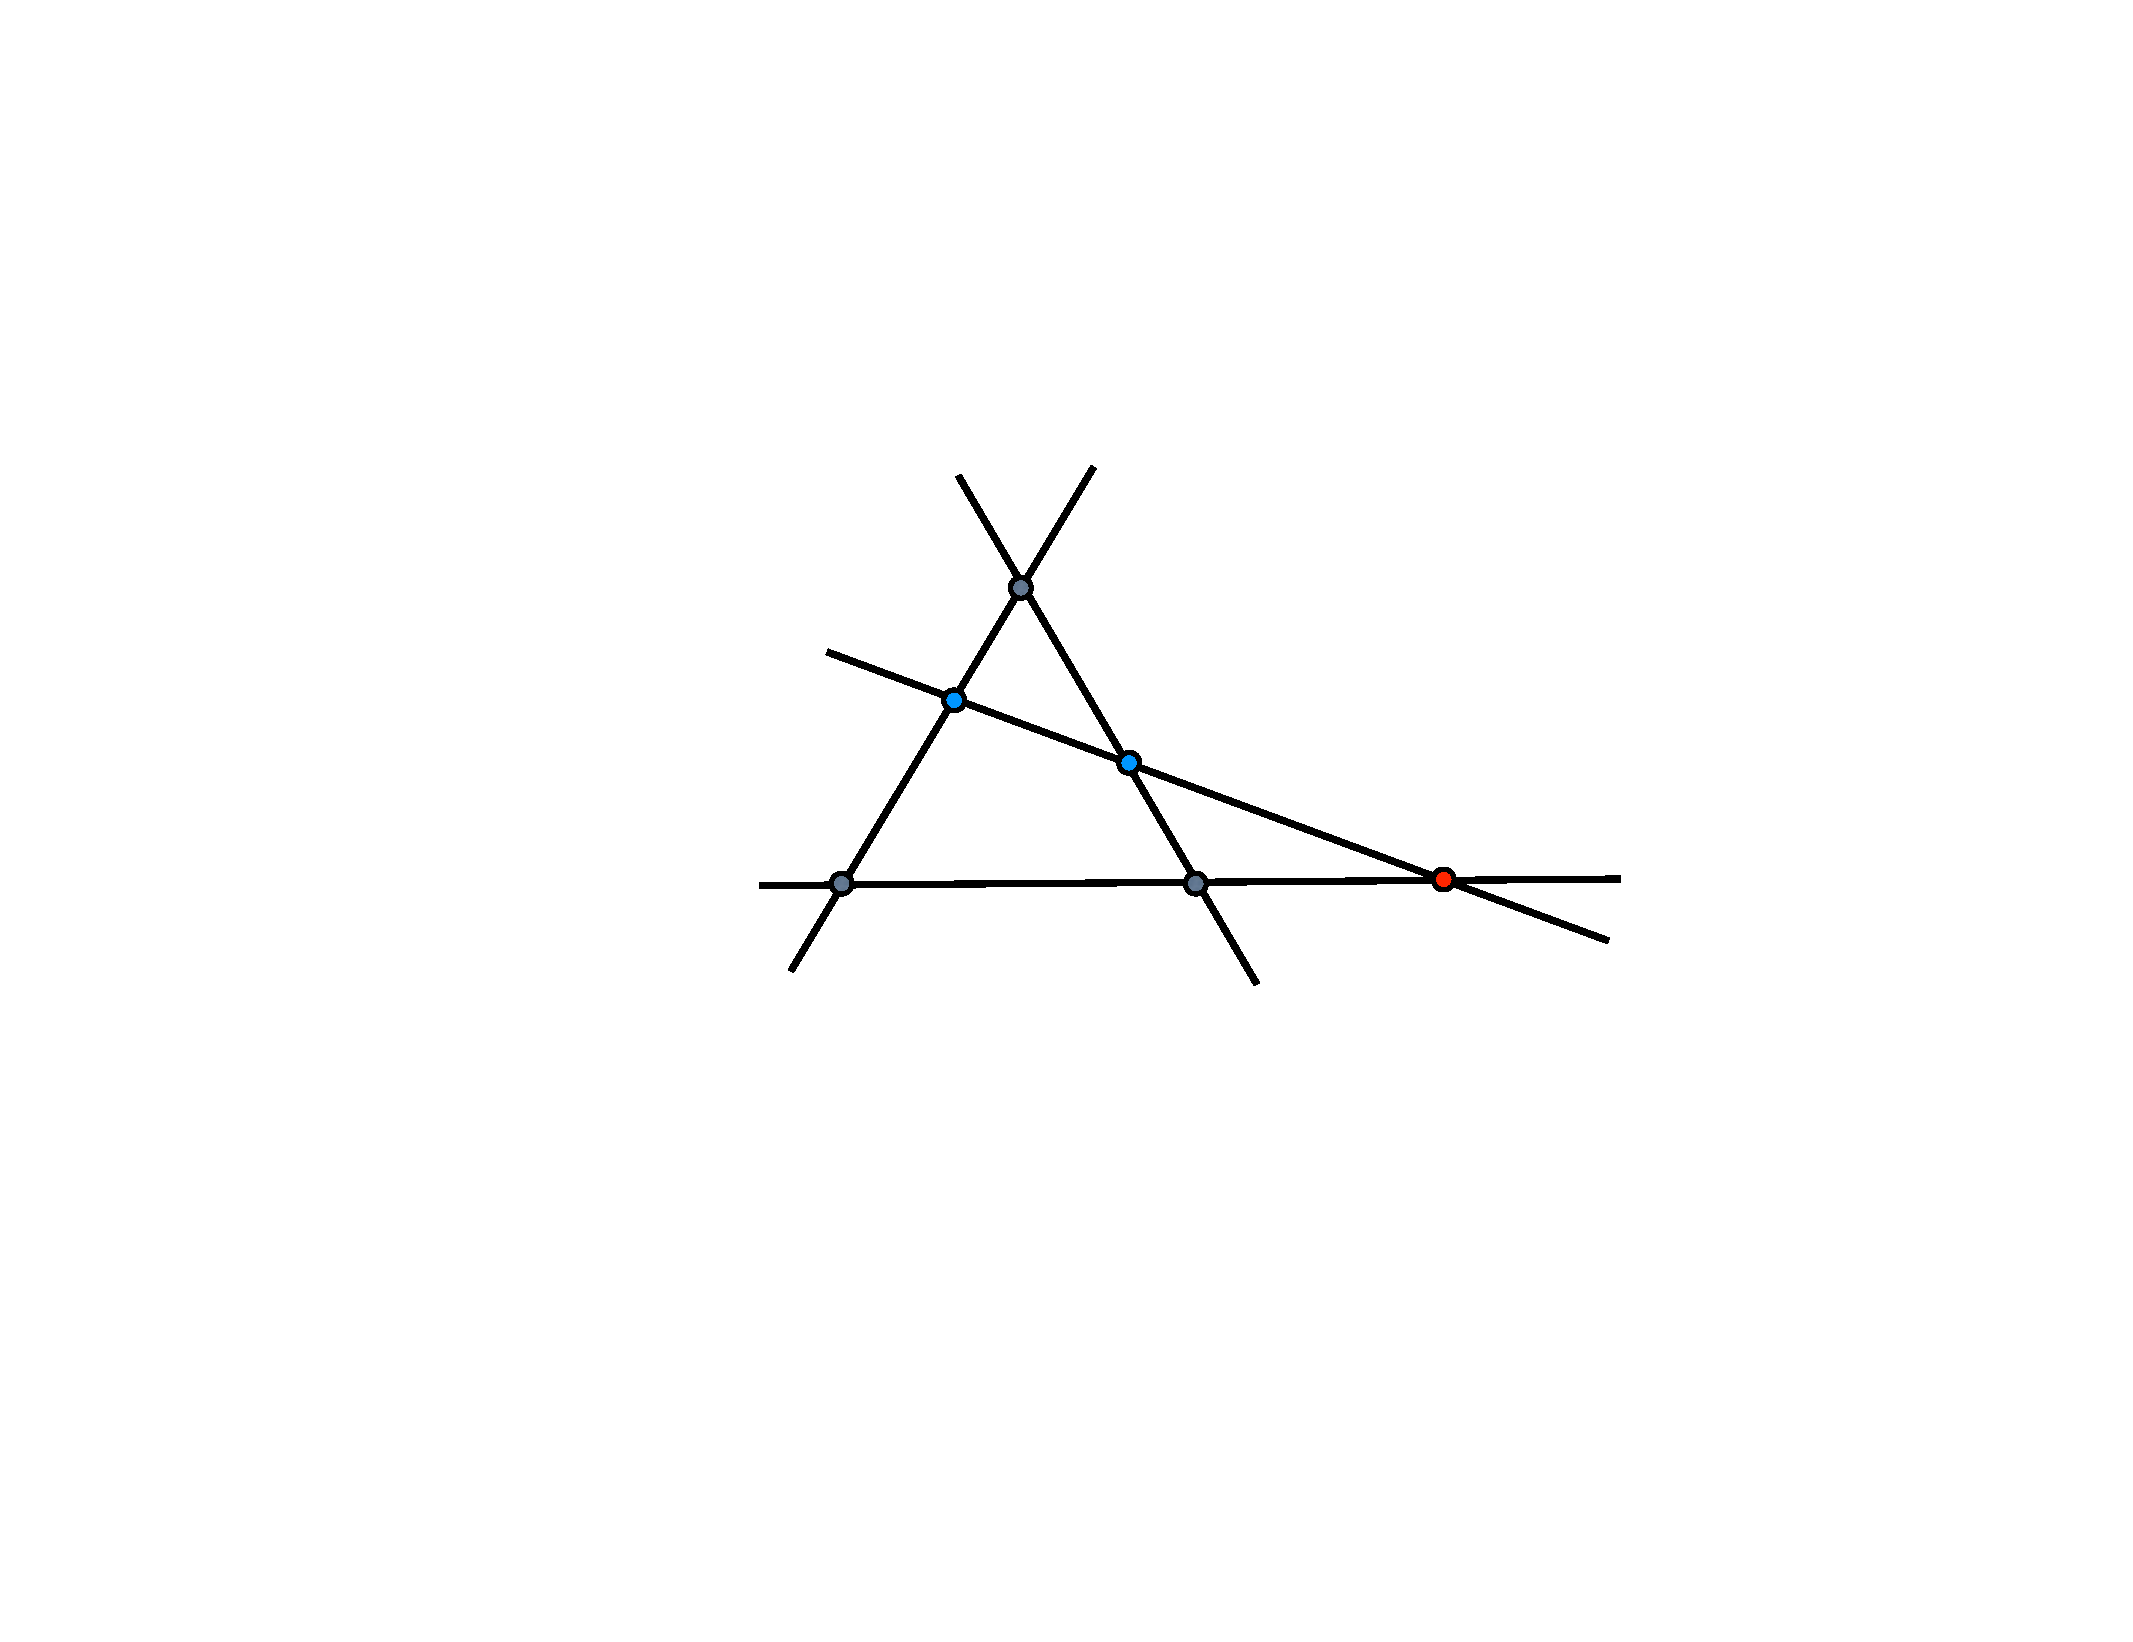
\includegraphics[width=4in]{Veblen.pdf}
\caption{Veblen's axiom}
\label{Veblen}
\end{center}
\end{figure} 

 The fourth one is necessary to exclude some special non-Desarguesian geometries.

Let me note that the division ring $K$ (an associative algebra with an addition $+$, a multiplication $\times$ and an inverse $x\to x^{-1}$) is constructed out of the symmetries of the geometry, i.e. of the automorphisms, or applications $X\to X$, $\mathcal{L}\to\mathcal{L}$, etc. which preserve the geometry. Without giving any details, let me illustrate the case of the standard real projective plane (where $K=\mathbb{R}$). The field structure on $\mathbb{R}$ is obtained by identifying $\mathbb{R}$ with a projective line $\ell$ with three points $0$, $1$ and $\infty$. The ``coordinate'' $x\in\mathbb{R}$ of a point $X\in\ell$ is identified with the cross-ratio $x=(X,1;0,\infty)$.
On Fig.~\ref{projplustimes} are depicted the  geometrical construction of the addition $X+Y$ and of the multiplication $X\times Y$ of two points $X$ and $Y$ on a line $\ell$.
\begin{figure}[h]
\begin{center}
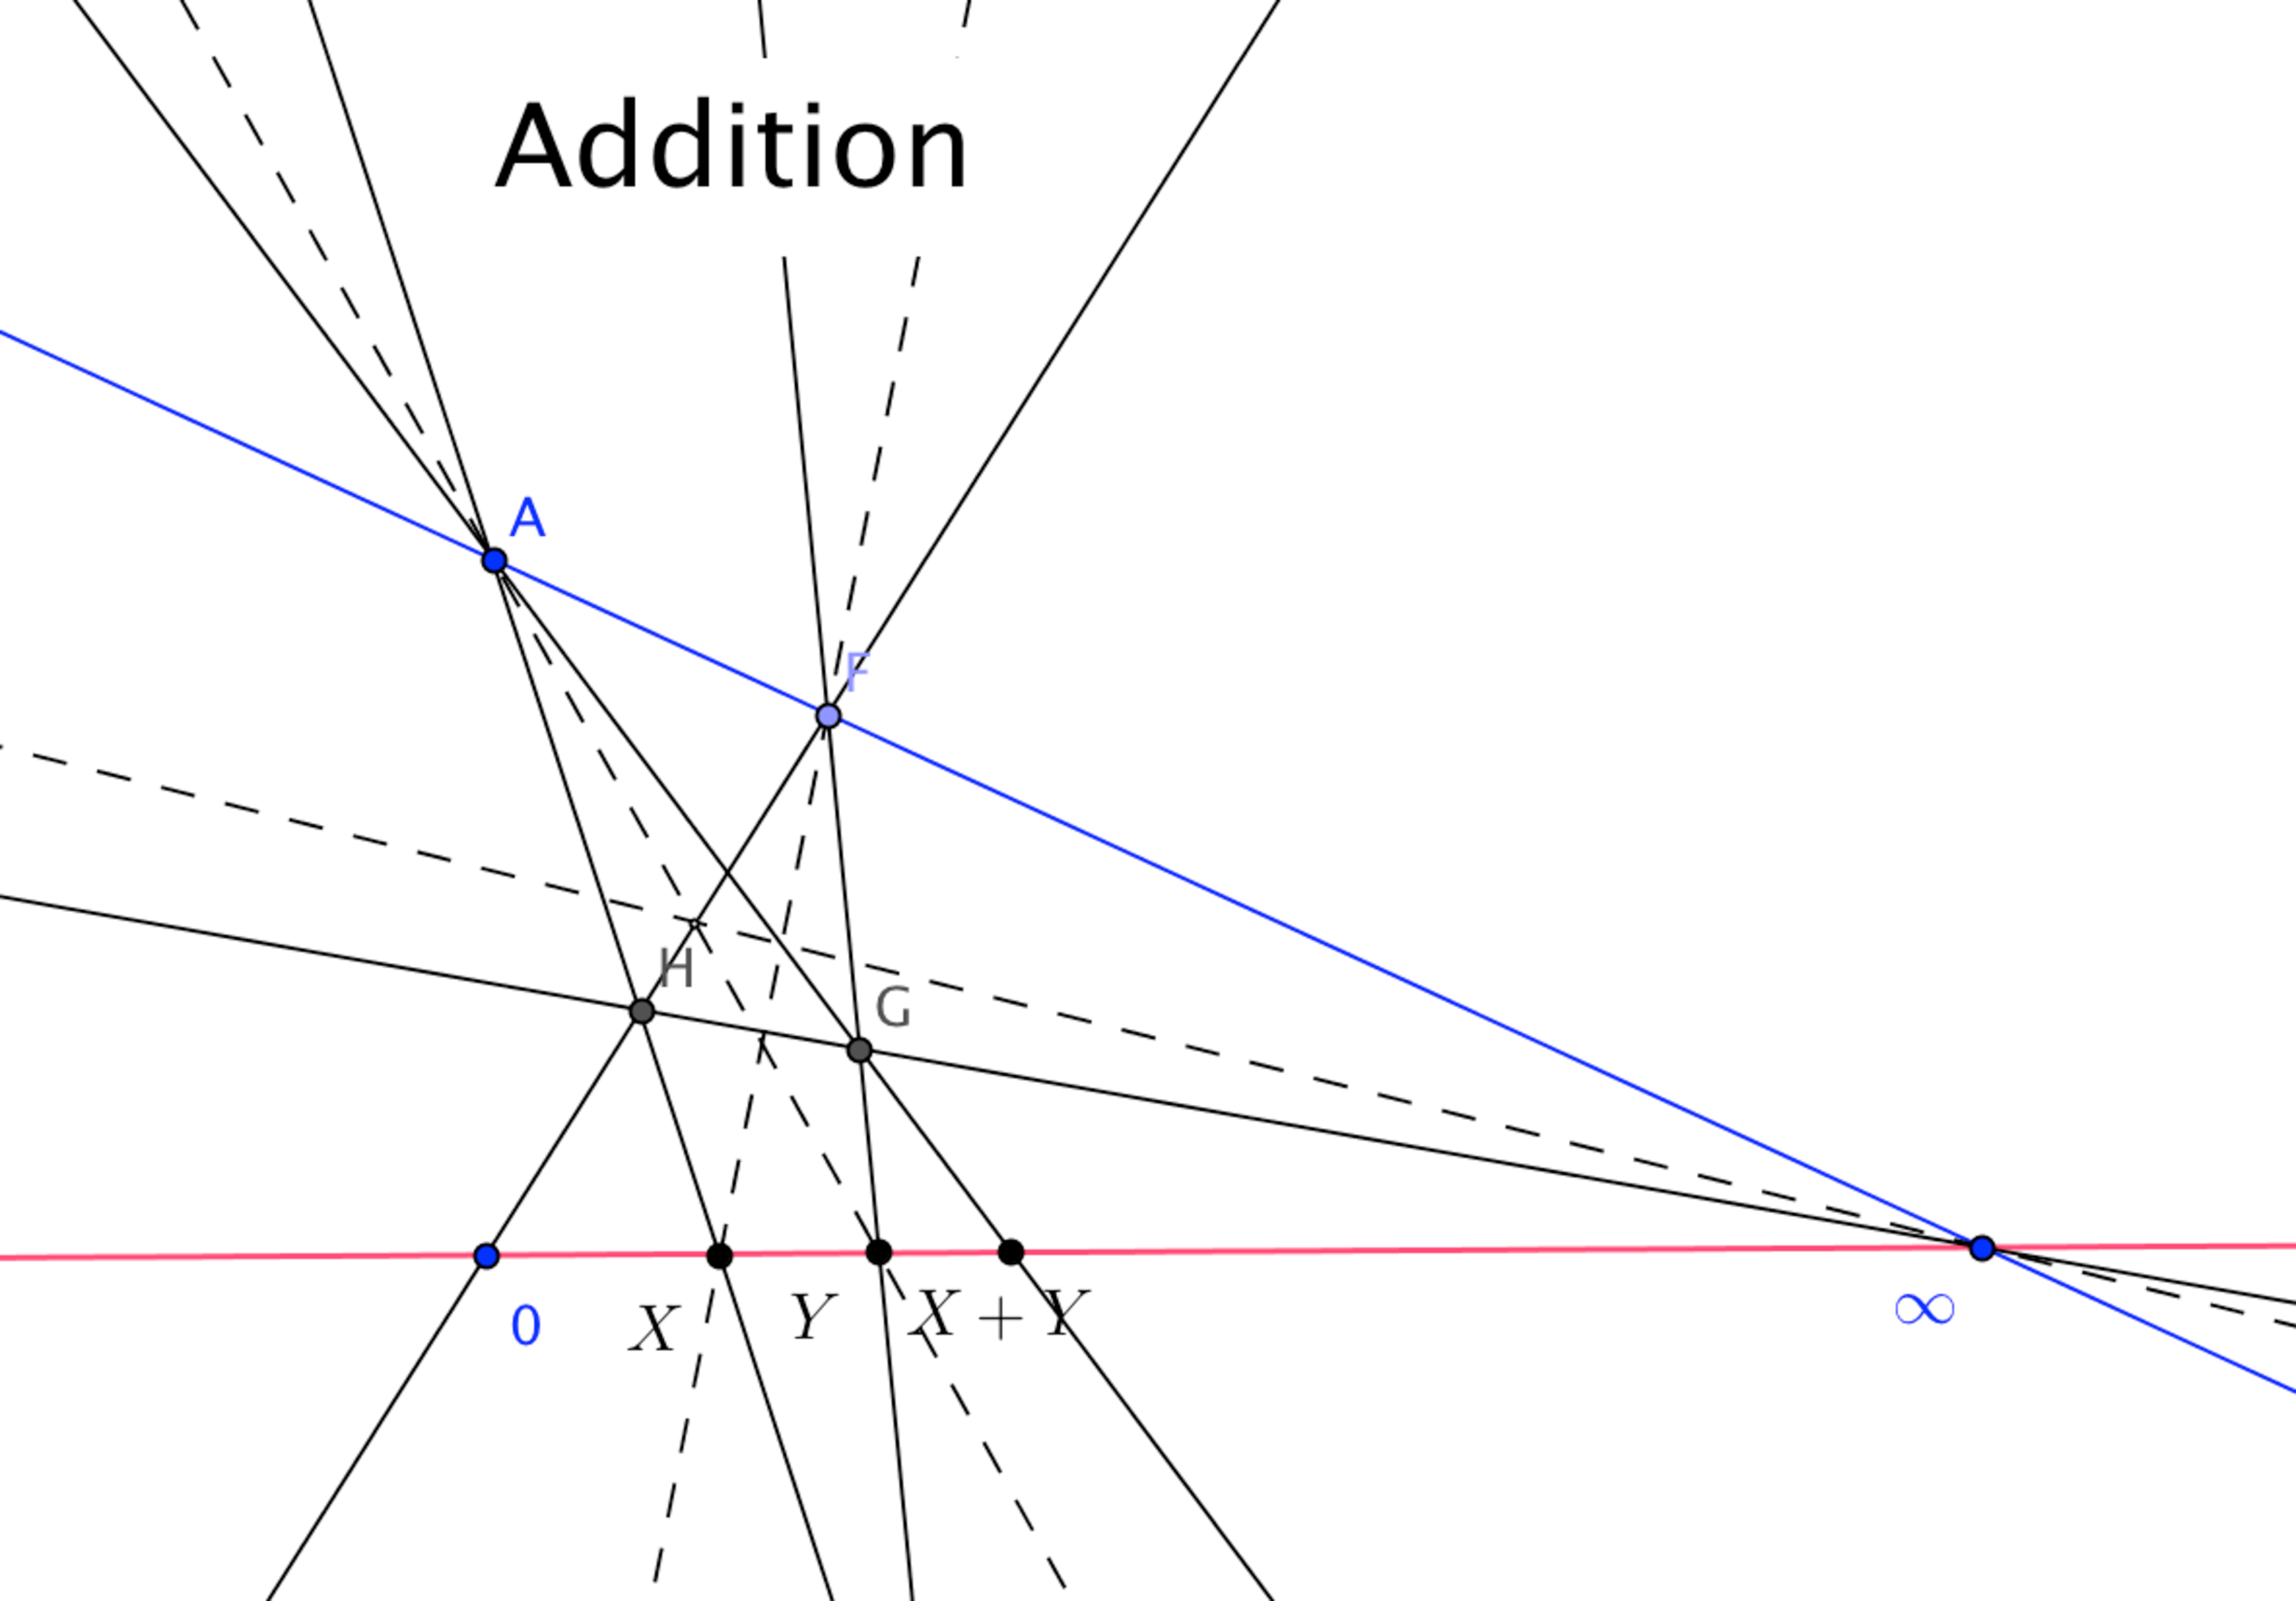
\includegraphics[width=2.99in]{addition.pdf}
\quad
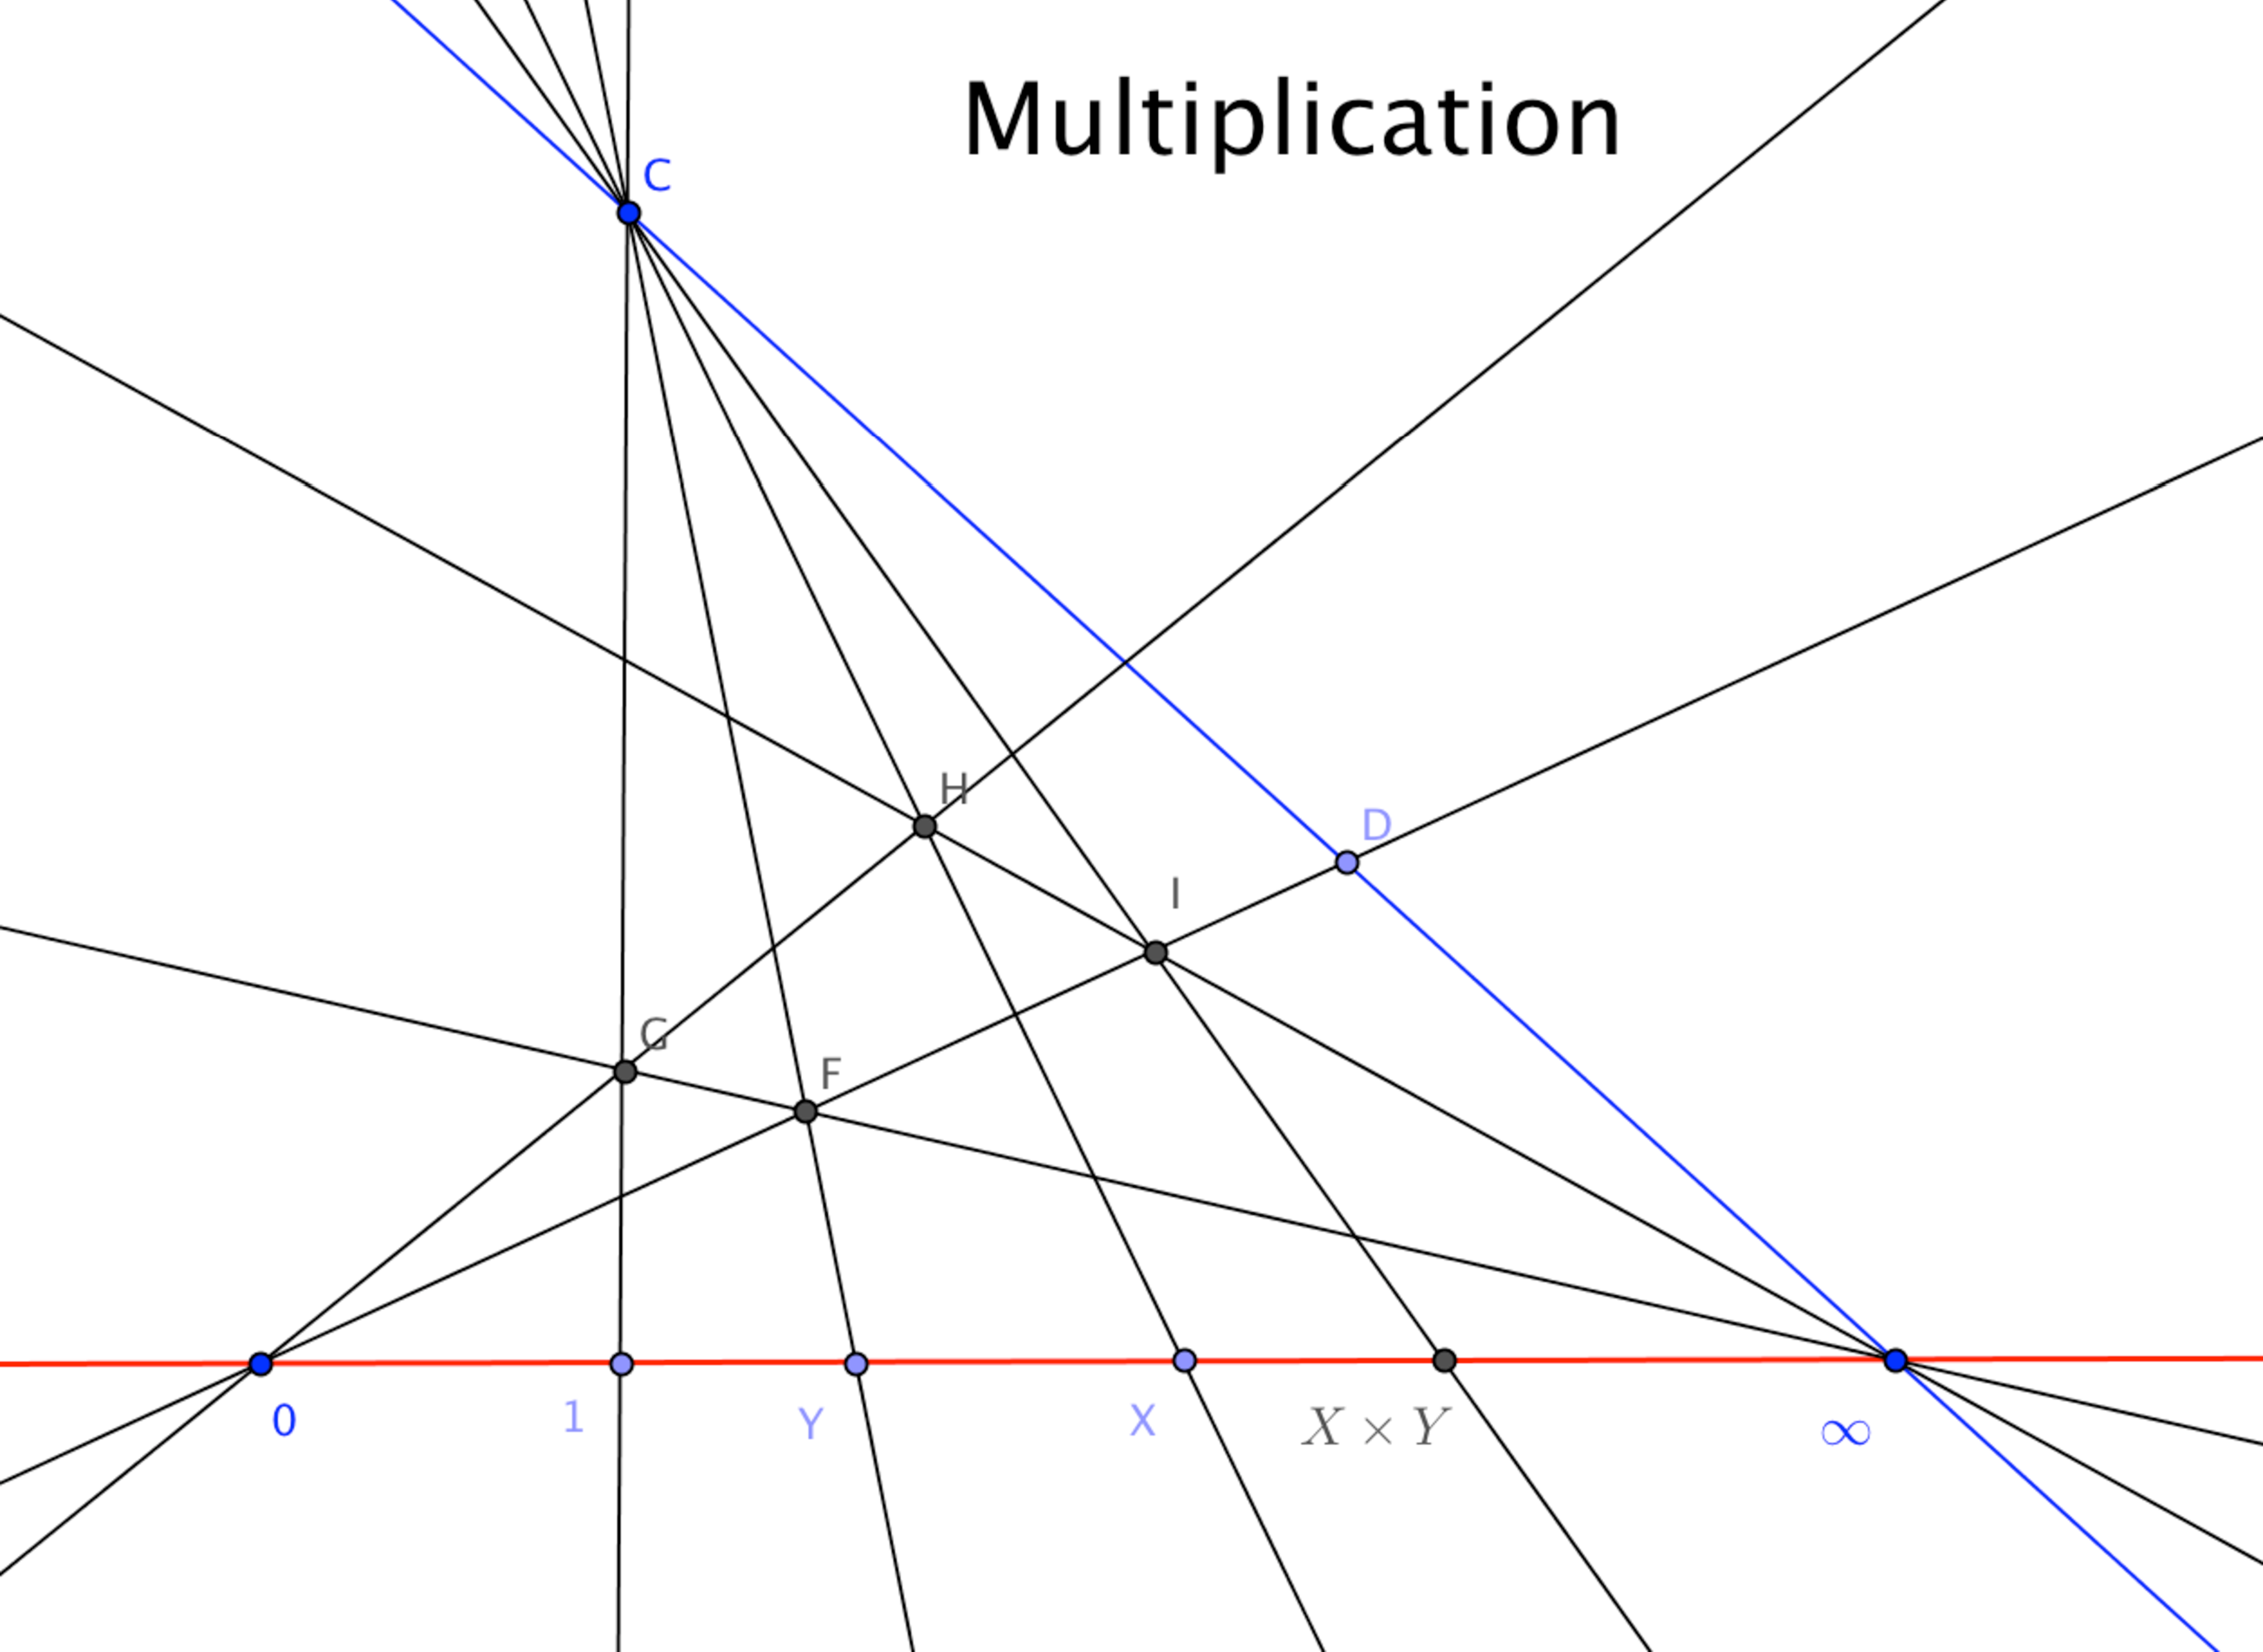
\includegraphics[width=2.99in]{multiplication.pdf}
\caption{Construction of $+$ and $\times$ in the  projective real plane}
\label{projplustimes}
\end{center}
\end{figure}

\subsection{The projective geometry of orthomodular AC lattices}

\subsubsection{The coordinatization theorem}
\index{Coordinatization theorem}
\index{Orthomodular lattice}
\index{Atomic lattice}
\index{Covering property}
\index{Division ring}
\index{Scalar product}

Similar ``coordinatization''  theorems hold for the orthomodular AC lattices that have been introduced in the previous section. The last axioms AC (atomicity and covering) play a similar role as the axioms of abstract projective geometry, allowing to define ``points'' (the atoms), lines, etc , with properties similar to the first 3 axioms of linear spaces. The difference with projective geometry is the existence of the orthocomplementation (the negation $\neg$) which allows to define an abstract notion of orthogonality $\perp$, and the specific property of weak-modularity (which will allows to define in a consistent way what are projections on closed subspaces).

Let me first state the main theorem


\paragraph{Theorem:}
Let $\mathcal{L}$ be a complete irreducible orthocomplemented AC lattice with length $>3$ (i.e. at least three 4 different levels of proposition $\emptyset\prec a\prec b\prec c\prec d\prec 1)$.
Then the ``abstract'' lattice $\mathcal{L}$ can be represented as the lattice $\mathcal{L}(V)$ of the closed subspaces of a left-module%
\footnote{A module is the analog of a vector space, but on a ring instead of a (commutative) field}
  $V$ on a division ring%
  \footnote{A division ring is the analog of a field, but without commutativity}
   $K$ with a Hermitian form $f$.
The ring $K$, the module $V$ and the form $f$ have the following properties:
\begin{itemize}
  \item The division ring $K$ has an involution $^*$  such that $(xy)^*=y^* x^*$
  \item The vector space $V$ has a non degenerate Hermitian (i.e. sesquilinear) form $f:\ V\times V \to K$
  \begin{equation}
\label{ }
\mathbf{a},\mathbf{b}\in V \ \ ,\ \ f(a,b)=\langle \mathbf{a}|\mathbf{b}\rangle\in K
  \quad,\quad \langle\mathbf{a}|\mathbf{b}\rangle=\langle\mathbf{b}|\mathbf{a}\rangle^*
\end{equation}
    \item The Hermitian form $f$ defines an orthogonal projection and associates to each linear subspace $M$ of $V$ its orthogonal $M^\perp$. 
    \begin{equation}
\label{ }
M^\perp=\{\mathbf{b}\in v:\ \langle\mathbf{b}|\mathbf{a}\rangle=0\ \ \forall\mathbf{a}\in M\}
\end{equation}
\item   The closed subspaces of $V$ are the subspaces $M$ such that $(M^\perp)^\perp=M$.
  \item The Hermitian form is orthomodular, i.e. for any closed subspace, $M^\perp+M=V$.
\item The OM structure $(\preceq\, ,\, \wedge\, ,\, ')$ on the lattice $\mathcal{L}$ is isomorphic to the standard lattice structure $(\subseteq\ ,\,\cap \,,\,\perp)$ (subspace of, intersection of, orthogonal complement of) over the space $\mathcal{L}(V)$ of closed linear subspaces of $V$.
\item Moreover, $V$ and $K$ are such that there is some element $a$ of $V$ with \og norm\fg{}  unity  $f(a,a)=1$ (where $1$ is the unit element of $K$).
\end{itemize} 

\medskip
I do not give the proof. I refer to the physics literature: ( \cite{BeltCassi81}  chapter 21, \cite{Piron64,Piron76}, and to the original mathematical literature  
\cite{BirkVNeumann36}
\cite{maeda1971theory}
\cite{Varadarajan1985}.

\medskip

Thus this theorem states that an OM AC lattice can be represented as the lattice of orthogonal projections over the closed linear subspaces of some ``generalized Hilbert space'' with a quadratic form defined over some non-commutative field $K$. This is very suggestive of the fact that Hilbert spaces are not abstract and complicated mathematical objects (as still sometimes stated), but are the natural objects to describe and manipulate ideal measurements in quantum physics.
In particular  the underlying ring $K$ and the algebraic structure of the space $V$ come out naturally from the symmetries of the lattice of propositions $\mathcal{L}$.

\subsubsection{Discussion: which division ring $K$?}
\label{sssRing}
The important theorem discussed before is very suggestive, but is not sufficient to ``derive'' standard quantum mechanics. 
The main question is which division algebra $K$ and which involution $^*$ and Hermitian form $f$ are physically allowed? Can one construct physical theories based on other rings than the usual $K=\mathbb{C}$ (or $\mathbb{R}$ or $\mathbb{H}$)?

The world of division rings is very large! The simplest one are finite division rings, where the first Wedderburn theorem implies that $K$ is a (product of) Galois fields $\mathbb{F}_p=\mathbb{Z}/\mathbb{Z}_p$ ($p$ prime). Beyond $\mathbb{C}$, $\mathbb{R}$ and $\mathbb{H}$, more complicated  ones are rings of rational functions $F(X)$, up to very large ones (like surreal numbers...), but still commutatives, to non-commutatives rings.

However, the requirements that $K$ has an involution, and that $V$ has a non degenerate hermitian form, so that $\mathcal{L}(V)$ is a OM lattice, put already very stringent constraints on $K$.
For instance, it is well known that finite fields like the $\mathbb{F}_p$ ($p$ prime) do not work. 
Indeed, it is easy to see that the lattice $\mathcal{L}(V)$ of the linear subspaces of the finite dimensional subspaces of the $n$-dimensional vector space $V=({\mathbb{F}_p})^n$ is not orthomodular and cannot be equipped with a non-degenerate quadratic form! Check with $p=n=3$!
But still many more exotic division rings $K$ than the standard $\mathbb{R}$, $\mathbb{C}$ (and $\mathbb{H}$) are possible at that stage
%(why not the class of surreal numbers for instance?)
.
\index{Galois field}

%\subsection{Le treillis orthomodulaire des propositions}
\subsection{Towards Hilbert spaces}
There are several arguments that point towards the standard solution: $V$ is a Hilbert space over $\mathbb{R}$, $\mathbb{C}$ (or $\mathbb{H}$).
However none is completely mathematically convincing, if most would satisfy a physicist.
Remember that real numbers are expected to occur in physical theory for two reasons. Firstly we are trying to compute probabilities $p$, which are real numbers. Secondly quantum physics must be compatible with the relativistic concept of space-time, where space (and time) is described by continuous real variables. Of course this is correct as long as one does not try to quantize gravity. 

We have not discussed yet precisely the structure of the states $\psi$, and which constraints they may enforce on the algebraic structure of propositions.
Remember that it is the set of states $\mathcal{E}$ which allows to discuss the partial order relation $\preceq$ on the set of propositions $\mathcal{L}$. Moreover states $\psi$ assign probabilities $\psi(a)\in[0,1]$ to propositions $a$, with the constraints that if $a\perp b$, $\psi(a\lor b)=\psi(a)+\psi(b)$.
Moreover the  propositions $a\in\mathcal{L}$ (projective measurements) define via the Sasaki orthogonal projections $\pi_a$ a set of transformations $\mathcal{L}\to\mathcal{L}$, which form  a so called Baer $^*$-semi group.
On the same time, propositions $a\in\mathcal{L}$ define mappings $\psi\to\psi_a$ on the states. 
Since as in the algebraic formalism, convex linear combinations of states are states, $\mathcal{E}$ generate a linear vector space $E$, and form a convex subset $\mathcal{E}\subset E$. 
%The transformations on states associated to propositions form  a so called Baer $^*$-semi group. 
Thus there is more algebraic structure to discuss than what I explained up to now. I refer to \cite{BeltCassi81}, chapters 16-19, for more details.
I shall come back to states when discussing Gleason's theorem in the next section.

Assuming some ``natural'' continuity or completeness conditions for the states leads to theorems stating that the division ring $K$ must contain the field of real numbers $\mathbb{R}$, hence is $\mathbb{R}$, $\mathbb{C}$ or $\mathbb{H}$, and that the involution $^*$ is continuous, hence corresponds to the standard involution $x^*=x$,  $x^*=\bar x$ or $x^*=x^\star$ respectively.
See \cite{BeltCassi81}, chapter 21.3.

 Another argument comes from an important theorem in the theory of orthomodular lattices, which holds for lattices of projections in infinite dimensional modules.


\paragraph{Sol{\`e}r's Theorem:} (Sol�r 1995) Let $\mathcal{L}=\mathcal{L}_K(V)$ be an irreducible OM AC lattice of compact linear suspaces in a left-module $V$ over a divison ring $K$, as discussed above. 
If there is an infinite family $\{v_i\}$ of orthonormal vectors in $V$ such that $\langle v_i|v_j\rangle=\delta_{ij} f$ with some $f\in K$ 
%(an infinite set of mutually compatible atoms in $\mathcal{L}$)
 then the division ring $K$ can only be $\mathbb{R}$, $\mathbb{C}$ or $\mathbb{H}$.
 \index{Soler's theorem}

\medskip
The proof of this highly non trivial theorem is given in \cite{Soler95}. It is discussed in more details in \cite{Holland95}.

%\par
\medskip

The assumptions of the theorem state that there an infinite set of mutually compatible atoms $\{a_i\}_{i\in I}$ in $\mathcal{L}$ (commuting, or causally independent elementary propositions $a_i$), and in addition that there is some particular symmetry between the generators $v_i\in V$ of the linear spaces (the lines or rays) of these propositions.

The first assumption is quite natural if we take into account space-time and locality in quantum physics.
Let me consider the case where the physical space in which the system is defined to be infinite (flat) space or some regular lattice, so that it can be separated into causally independent pieces $\mathcal{O}_\alpha$ (labelled by $\alpha\in\Lambda$ some infinite lattice). See for instant Fig.~\ref{StrCauDia}. 
It is sufficient to have one single proposition $a_\alpha$ relative to each $\mathcal{O}_\alpha$ only (for instance ``there is one particle in $\mathcal{O}_\alpha$'') to build an infinite family of mutually orthogonal propositions $b_\alpha=a_\alpha\wedge(\bigwedge_{\beta\neq\alpha}\neg a_\beta)$ in $\mathcal{L}$. 
Out of the $b_\alpha$, thanks to the atomic property (A), we can extract an infinite family of orthogonal atoms $c_\alpha$.
\begin{figure}[h]
\begin{center}

\includegraphics[width=4in]{StringDiamonds.pdf}
\caption{A string of causal diamonds (in space-time)}
\label{StrCauDia}
\end{center}
\end{figure}

However this does not ensure the second assumption: the fact that the corresponding $v_i\in V$ are orthonormals. The group of space translations $\mathfrak{T}$ must act as a group of automorphism on the lattice of linear subspaces $\mathcal{L}=\mathcal{L}_K(V)$ (a group of automorphisms on a OC lattice $\mathcal{L}=\mathcal{L}_K(V)$ is a group of transformations which preserves the OC lattice structure  $(\preceq\,,\, \wedge\,,\, ')$ or equivalently $(\subseteq\, ,\ \cap\, ,\, \perp)$). There must correspond an action (a representation) of the translation group $\mathfrak{T}$ on the vector space $V$, and on the underlying field $K$. If the action is trivial the conditions of Soler's theorem are fulfilled, but this is not ensured a priori. See for instance \cite{Casinelli-Lahti-2012} for a recent discussion of symmetries in orthomodular geometries. However I am not aware of a counterexample where a non standard orhomodular geometry (i.e. different from that of a Hilbert space on $\mathbb{C}$ (or $\mathbb{R}$) carries a representation of a ``physical'' symmetry group such as the Poincar� or the Galilean group of space-time transformations (representations of these groups should involves the field of real numbers $\mathbb{R}$ in some form).
\index{Poincar� invariance}
\index{Hilbert space}


From now on we assume that a quantum system may indeed be described by projectors in a real or complex Hilbert space.

One last remark. The coordinatization theorem depends crucially on the fact that the OM lattice $\mathcal{L}$ is atomic, hence contain minimal propositions (atoms). They are the analog of minimal projectors in the theory of operator algebras. Hence the formalism discussed here is expected to be valid mathematically to describe only type I  von Neumann algebras.
I shall not elaborate further.


%\section{Observables, states, Gleason's theorem and the Born rule}
\section{Gleason's theorem and the Born rule}

\subsection{States and probabilities}
\index{State}
\index{Probabilities}
In the presentation of the formalism we have not put emphasis on the concept of states, although states are central in the definition of the causality order relation $\preceq$ and  of the orthocomplementation $\ '$.
We recall that to each state $\psi$ and to each proposition $a$ is associated the probability $\psi(a)$ for $a$ to be found true on the state $\psi$.
In other word, states are probability measures on the set of propositions, compatible with the causal structure.
As already mentionned, the lattice structure of propositions can be formulated from the properties of the states on $\mathcal{L}$. 


At that stage we have almost derived the standard mathematical formulation of quantum mechanics. 
Proposition (yes-no observables) are represented by othonormal projectors on a Hilbert space $\mathcal{H}$. Projectors on pure states corresponds to projectors on one dimensional subspaces, or rays of $\mathcal{H}$ so the concept of pure states is associated to the vectors of $\mathcal{H}$.

Nevertheless it remains to understand which are the consistent physical states, and what are the rules which determine the probabilities for a proposition $a$ to be true in a state $\psi$, in particular in a pure state. 
We remind that the states are in fact characterized by these probability distributions $a\to\psi(a)$ on $\mathcal{L}$.
Thus states must form a convex set of functions $\mathcal{L}\to [0,1]$ and by consistency with the OM structure of $\mathcal{L}$ they must satisfy four conditions. These conditions define ``quantum probabilities''

\paragraph{Quantum probabilities:}
\begin{align}
\label{psicond1}
(1)\qquad    & \psi(a)\in [0,1]  \\
\label{psicond1b}
(2)\qquad    &  \psi(\emptyset)=0\ , \quad\psi(\mathbf{1})=1\\
\label{psicond1c}
(3)\qquad    & a\neq b\ \implies\ \exists\, \psi\ \text{such that}\ \psi(a)\neq\psi(b)\\
\label{psicond1d}
(4)\qquad    & a\perp b\ \implies\ \text{}\quad \psi(a\vee b)=\psi(a)+\psi(b)
\end{align}
Conditions (1) and (2) are the usual normalization conditions for probabilities.
Condition (3)  means that observables are distinguishable by their probabilities.
Condition (4)  is simply the fact that if $a$ and $b$ are orthogonal, they generate a Boolean algebra, and the associated probabilities must satisfy the usual sum rule.
These conditions imply in particular that for any state $\psi$,  $\psi(\neg a)=1-\psi(a)$, and that if $a\preceq b$, then $\psi(a)\le\psi(b)$, as we expect.

It remains to understand if and why all states $\psi$  can be represented by density matrices $\rho_\psi$, and the probabilities for propositions $\mathbf{a}$ given by $\psi(\mathbf{a})=\tr(\rho_\psi P_\mathbf{a})$, where $P_\mathbf{a}$ is the projector onto the linear -subspace associated to the proposition $\mathbf{a}$.
This is a consequence of a very important theorem in operator algebras, Gleason's theorem \cite{Gleason57}.

\subsection{Gleason's theorem}
\label{ssGleason}
\index{Gleason's theorem}
It is easy to see that to obtain quantum probabilities that satisfy the conditions \ref{psicond1}- \ref{psicond1d}, it is sufficient to consider atomic propositions, i.e. projections onto 1 dimensional subspaces (rays) generated by vectors $\vec e=|e\rangle$ (pure states) of the Hilbert space $\mathcal{H}$. Indeed, using \ref{psicond1d}, the probabilities for general projectors can be reconstructed (by the usual sum rule) from the probabilities for projections on rays. Denoting since there is no ambiguity for a state $\psi$ the probability for the atomic proposition $\mathbf{e}$ represented by the projection $P_{\vec e}$ onto a vector $\vec e=|\vec e\rangle\in\mathcal{H}$ as
\begin{equation}
\label{}
\psi(\mathbf{e})=\psi(P_{\mathbf{ e}})=\psi(\vec e)
\qquad
P_{\vec e}=|\vec e\rangle\langle\vec e|\ =\ \text{projector onto\ }\vec e
\end{equation}
The rules  \ref{psicond1}- \ref{psicond1d} reduces to the conditions.

\paragraph{Quantum probabilities for projections on pure states:}
For any states $\psi$, the function $\psi(\vec e)$ considered as a function on the ``unit sphere'' of the rays over the Hilbert Space $\mathcal{H}$ (the projective space) $\mathcal{S}=\mathcal{H}^*/K^*$  must satisfy
\begin{align}
\label{frame1a}
  (1)\qquad   &   \psi(\vec e)=\psi(\lambda\vec e)\quad\text{for any\ }\lambda\in K\ \text{such that\ } |\lambda |=1\\
 \label{frame1b} (2) \qquad &   0\le \psi(\vec e)\le 1\\
 \label{frame1c}(3)\qquad   &  \text{For any complete orthonormal basis of}\  \mathcal{H},\   \{\vec e_i\},\ \text{one has}\ \sum_i\psi(\vec e_i)=1
\end{align}

Gleason's theorem states the fundamental result that any such function is in one to one correspondence with a density matrix.

\paragraph{Gleason's theorem:} \ \\
If the Hilbert space $\mathcal{H}$ over $K=\mathbb{R}$ or $\mathbb{C}$ is such that
\begin{equation}
\label{ }
\dim(\mathcal{H})\ge 3
\end{equation}
then any function $\psi$ over the unit rays of $\mathcal{H}$ that satisfies the three conditions \ref{frame1a}--\ref{frame1c} is of the form
\begin{equation}
\label{frame2qform}
\psi(\vec e)=(\vec e \cdot \rho_\psi \cdot\vec e) =\langle \vec e|\rho_\psi |\vec e\rangle
\end{equation}
where $\rho_\psi$ is a positive quadratic form (a density matrix) over $\mathcal{H}$ with the expected properties for a density matrix
\begin{equation}
\label{ }
\rho_\psi=\rho_\psi^\dagger\quad,\qquad \rho_\psi\ge 0\quad,\qquad \tr(\rho_\psi)=1
\end{equation}
Reciprocally, any such quadratic form defines a function $\psi$ with the three properties \ref{frame1a}--\ref{frame1c}.

\medskip\medskip
Gleason's theorem is fundamental. As we shall discuss more a bit later, it implies the Born rule. It is also very important when discussing (and excluding a very general and most natural class of) hidden variables theories. So let us discuss it a bit more, without going into the details of the proof.

\subsection{Principle of the proof} % \ \\
%\paragraph{Principle of the proof of Gleason's theorem:}  \ \\

The theorem is remarkable since there are non conditions on the regularity or measurability of the function $\psi$. In the original derivation by Gleason \cite{Gleason57} he considers real ``frame functions'' $f$ of weight $W$ over $\mathcal{H}^*=\mathcal{H}\backslash \{0\}$ such that
\begin{align}
\label{frame2a}
  (1)\qquad   &   f(\vec e)=f(\lambda\vec e)\quad\text{for any\ }\lambda\neq 0 \in K\\
 \label{frame2b} (2) \qquad &   f\quad\text{is bounded}\\
 \label{frame2c}(3)\qquad   &  \text{For any complete orthonormal basis of}\  \mathcal{H},\   \{\vec e_i\},\ \sum_i f(\vec e_i)=W=\text{constant}
\end{align}
and proves that such a function must be of the form \ref{frame2qform}
\begin{equation}
\label{ }
f(\vec e)=(\vec e{\cdot}Q{\cdot}\vec e)\quad,\qquad Q\quad \text{quadradic form such that\quad } \tr(Q)=W
\end{equation}
It is easy to see that this is equivalent to the theorem as stated above, since one can add constants and rescale the functions $f$ to go from \ref{frame2a}--\ref{frame2c} to \ref{frame1a}--\ref{frame1c}. The original proof goes into three steps

\begin{enumerate}
  \item Real Hilbert space, $\dim(\mathcal{H})=3$
  % ($\mathcal{H}=\mathbb{R}^3$) 
  and $f$ a continuous frame function $\implies$ the theorem\\
  This is the easiest part, involving some group theory.
   Any frame function $f$ is a real function on the unit two dimensional sphere $\mathcal{S}_2$ and if continuous it is square summable and can be decomposed into  spherical harmonics 
  \begin{equation}
\label{fYlm}
f(\vec n)=\sum_{l,m} f_{l,m} Y^{m}_{l}(\theta,\varphi)
\end{equation}
The theorem amounts to show that if $f$ is a frame function of weight $W=0$, then only the $l=2$ components of this decomposition \ref{fYlm} are non zero. Some representation theory (for the SO(3) rotation group) is enough.
Any orthonormal (oriented) basis $(\vec e_1,\vec e_2,\vec e_3)$ of $\mathbb{R}^3$ is obtained by applying a rotation $R$ to the basis $(\vec e_x,\vec e_y,\vec e_z)$. Thus one can write
\begin{equation}
\label{fbasis}
f(\vec n_1)+f(\vec n_2)+f(\vec n_3)=\sum_l \sum_{m,m'}  f_{l,m}\  D^{(l)}_{m,m'}(R)\  V^{(l)}_{m'}
\end{equation}
with the $D^{(l)}_{m,m'}(R)$ the Wigner $D$ matrix for the rotation $R$, and the $V^{(l)}_{m'}$ the components of the vectors $\vec V^{(l)}$ in the spin $l$ representation of $SO(3)$, with components
%A bit of group representation theory (for the SO(3) rotation group) shows that this is equivalent to state that the vectors  $\vec V^{(l)}$ in the spin $l$ representation of $SO(3)$, with components
\begin{equation}
\label{ }
\vec V^{(l)}=\{V^{(l)}_m\}\quad,\qquad V^{(l)}_m= Y_{l,m}(0,0)+Y_{l,m}(\pi/2,0)+Y_{l,m}(\pi/2,\pi/2)
\end{equation}
If $f$ is a frame function of weight $W=0$, the l.h.s. of \ref{fbasis} is zero for any $R\in\mathrm{SO(3)}$. This implies that for a given $l$, the coefficients $f_{lm}$ must vanish if the vector $\vec V^{(l)}\neq 0$, but are free if $\vec V^{(l)}=0$.
An explicit calculation shows that indeed
\begin{equation}
\label{ }
\vec V^{(l)}\ \begin{cases}
      \neq 0& \text{if}\ l\neq 2, \\
      =0 & \text{if}\ l=2.
\end{cases}
\end{equation}
This establishes the theorem in case (1).

  \item Real Hilbert space, $\dim(\mathcal{H})=3$
  % ($\mathcal{H}=\mathbb{R}^3$) 
  and $f$ any  frame function $\implies$ $f$ continuous.\\
  This is the most non-trivial part: assuming that the function is bounded, the constraint \ref{frame2c} is enough to imply that the function is continuous! It involves a clever use of spherical geometry and of the frame identity $\sum\limits_{i=1,2,3}f(\vec e_i)=W$. 
The basic idea is to start from the fact that since $f$ is bounded, it has a lower bound $f_{min}$ which can be set to 0. Then for any $\epsilon>0$, take a vector $\vec n_0$ on the sphere such that $|f(\vec n_0)-f_{min}|<\epsilon$. It is possible to show that there is a neibourhood $\mathcal{O}$ of $\vec n_0$ such that $|f(\vec n_1)-f(\vec n_2)|< C\, \epsilon$ for any $\vec n_1$ and  $\vec n_2\in\mathcal{O}$. $C$ is a universal constant. It follows that the function $f$ is continuous at its minimum! Then it is possible, using rotations to show that the function $f$ is continuous at any points on the sphere.

  \item Generalize to $\dim(\mathcal{H})>3$ and to complex Hilbert spaces.\\
This last part is more standard and more algebraic. Any frame function $f(\vec n)$ defined on unit vectors $\vec n$ such that $\| \vec n\|=1$ may be extended to a quadratic function over vectors $f(\vec v)=\|\vec v\|^2 f(\vec v/\|\vec v\|)$.

For a real Hilbert space with dimension $d>3$, the points (1) and (2) implies that the restriction of a frame function $f(\vec n)$ to any 3  dimensional subspace is a quadratic form $f(\vec v)=(\vec v{\cdot}Q{\cdot}\vec v)$.
A simple and classical theorem by Jordan and von Neumann shows that this is enough to define a global real quadratic form $Q$ on the whole Hilbert space $\mathcal{H}$ through the identity
$2(\vec x{\cdot}Q{\cdot}\vec y)=f(\vec x+\vec y)-f(\vec x-\vec y)$.

For complex Hilbert spaces, the derivation is a bit more subtle. One can first apply the already obtain results to the restriction of frame functions over real submanifolds of $\mathcal{H}$ (real submanifolds are real subspaces of $\mathcal{H}$ such that ($\vec x{\cdot}\vec y)$ is always real). One then extends the  obtained real quadratic form over the real submanifolds to a complex quadratic form on $\mathcal{H}$.

\end{enumerate}

\subsection{The Born rule}
\index{Born rule}
\index{Density matrix}
\index{Pure state}
The Born rule is a simple consequence of Gleason theorem.
Indeed, any state (in the general sense of statistical state) corresponds to a positive quadratic form (a density matrix) $\rho$ and given a minimal atomic proposition, which corresponds to a projector $P=|\vec a\rangle\langle\vec a|$ onto the ray corresponding to a single vector (pure state) $|\vec a\rangle$, the probability $p$ for $P$ of being true is
\begin{equation}
\label{ }
p=\langle P\rangle=\tr(\rho P)=\langle \vec a|\rho|\vec a\rangle
\end{equation}
The space of states $\mathcal{E}$ is thus the space of (symmetric) positive density matrices with unit trace 
\begin{equation}
\label{ }
\text{space of states}\ =\ \mathcal{E}=\{\rho:\ \rho=\rho^\dagger,\ \rho\ge 0\ , \tr(\rho)=1\}
\end{equation}
It is a convex set. Its extremal points, which cannot be written as a linear combination of twi different states, are the pure states of the system, and are the density matrices of rank one, i. e. the density matrices which are themselves projectors onto a vector $|\psi\rangle$ of the Hilbert space.
\begin{equation}
\label{ }
\rho\ =\ \text{pure state}\quad\implies\quad \rho=|\psi\rangle\langle\psi |
\quad,\quad \|\psi\|=1
\end{equation}
One thus derives the well known fact that the pure states are in one to one correspondence with the vectors (well... the rays) of the Hilbert space $\mathcal{H}$ that was first introduced from the bassc observables of the theory, the elementary atomic propositions (the projectors $P$).
Similarily, one recovers the simplest version of the Born rule: the probability to measure a pure state $|\varphi\rangle$ into another pure state $|\psi\rangle$ (to ``project''  $|\varphi\rangle$ onto $|\psi\rangle$) is the square of the norm of the scalar product
\begin{equation}
\label{ }
p(\varphi\to\psi)\ =\ |\langle\varphi|\psi\rangle|^2
\end{equation}



\subsection{Physical observables}
\index{Physical observable}
One can easily reconstruct the set of all physical observables, and the whole algebra of observables $\mathcal{A}$ of the system.
I present the line of the argument, without any attempt of mathematical rigor.

Any ideal physical mesurement of some observable $O$ consists in fact in taking a family of mutually  orthogonal propositions $a_i$, i.e. of commuting symmetric projectors $P_i$ on $\mathcal{H}$ such that
\begin{equation}
\label{ }
P_i^2=P_i\ ,\quad P_i=P_i^*\ ,\quad P_i P_j=P_j P_i=0\ \ \text{if}\ i\neq j
\end{equation}
%assigning a \emph{real number} $o_i$ to each proposition $a_i$ (the value of the observable $O$ if $a_i$ is found true, 
performing all the tests (the order is unimportant since the projectors commute) and 
assigning a \emph{real number} $o_i$ to the result of the measurement (the value of the observable $O$) if $a_i$ is found true (this occurs for at most one $a_i$) and zero otherwise.
% and summing the $o_i$ when the $a_i$ are found to be true.
In fact one should take an appropriate limit when the number of $a_i$ goes to infinity, but I shall not discuss these important points of mathematical consistency.
If you think about it, this is true for any imaginable measurement (position, speed, spin, energy, etc.).
The resulting physical observable $O$ is thus associated to the symmetric operator
\begin{equation}
\label{ }
O=\sum_i o_i P_i
\end{equation}
This amounts to the spectral decomposition of symmetric operators in the theory of algebras of operators.
\index{Spectral decomposition}

Consider a system in a general state given by the density matrix $\rho$.
From the general rules of quantum probabilities, the probability to find the value $o_i$ for the measurement of the observable $O$ is simply the sum of the probabilities to find the system in a eigenstate of $O$ of eigenvalue $o_i$, that is
\begin{equation}
\label{ }
p(O\to o_i)= \tr(P_i\rho)
\end{equation}
and for a pure state $|\varphi\rangle$ it is simply 
\begin{equation}
\label{ }
\langle \varphi|P_i|\varphi\rangle= |\langle\varphi|\varphi_i\rangle|^2
\quad,\qquad |\varphi_i\rangle ={1\over \|P_i|\varphi\rangle\|}\, P_i | \varphi \rangle
\end{equation}
Again the Born rule!
\index{Born rule}
The expectation value for the result of the measurement of $O$ in a pure state $\psi_a$ is obviously 
%\begin{equation}
%\label{ }
%P(a,O)=v_a{\cdot} O{\cdot} v_a
%\end{equation}
%or equivalently in standard notations
\begin{equation}
\label{ }
\mathbb{E}[O;\psi]\ =\ \langle O\rangle_\psi= \sum_i o_i \ p(O\to o_i)\ =\ \sum_i o_i \langle\psi | P_i|\psi\rangle\ =\  \langle\psi | O |\psi\rangle
\end{equation}
This is the standard expression for expectation values of physical observables as diagonal matrix elements of the corresponding operators. Finally for general (mixed) states one has obviousy
\begin{equation}
\label{ }
\mathbb{E}[O;\rho]\ =\ \langle O\rangle_\rho= \sum_i o_i \, p(O\to o_i)\ =\ \sum_i o_i \,\tr(P_i \rho)\ =\  \tr( O \rho)
\end{equation}

We have seen that the pure states generate by convex combinations the convex set $\mathcal{E}$ of all (mixed) states $\psi$ of the system. 
Similarily the symmetric operators $O=O^\dagger$ generates (by operator multiplication and linear combinations) a C$^*$-algebra $\mathcal{A}$ of bounded operators $\mathcal{B}(\mathcal{H})$ on the Hilbert space $\mathcal{H}$.
States are normalized positive linear forms on $\mathcal{A}$ and we are back to the standard algebraic formulation of quantum physics.
The physical observables generates an algebra of operators, hence an abstract algebra of observables, as assumed in the algebraic formalism.
We refer to the section about the algebraic formalism for the arguments for preferring complex Hilbert spaces to real or quaternionic ones.

\section{Discussion}
This was a sketchy and partial introduction to the quantum logic approach for the formulation of the principle of quantum mechanics. 
I hope to have shown its relation with the algebraic formulation. It relies  on the concepts of states and of observables as the algebraic formulation. However the observables are limited to the physical subset of yes/no proposition, corresponding to ideal projective measurements, without assuming a priori some algebraic structure between non-compatible  propositions (non-commuting observables in the algebraic framework). I explained how the minimal set of axioms on these propositions and their actions on states, used in the quantum logic approach, is related to the physical concepts of causality, reversibility and separability/locality.
The canonical algebraic structure of quantum mechanics comes out from the symmetries of the ``logical structure'' of the lattice of propositions.
The propositions corresponding to ideal projective measurements are realized on orthogonal projections on a (possibly generalized) Hilbert space.
Probabilities/states are given by quadratic forms, and the Born rule follows from the logical structure of quantum probabilities through Gleason's theorem.

\index{von Neumann algebra}
\index{Bipartite system}
\index{Tensor product}
This kind of approach is of course not completely foolproof. We have seen that the issue if the possible division algebras $K$ is not completely settled. The strong assumptions of atomicity and covering are essential, but somehow restrictive compared to the algebraic approach (type II and III von Neumann algebras). It is sometime stated that it cannot treat properly the case of a system composed of two subsystems since there is no concept of ```tensorial product'' of two OM-AC lattices as there is for Hilbert spaces and operator algebras. Note however that one should in general always think about multipartite systems as parts of a bigger system, not the opposite! Even in the algebraic formulation it is not known in the infinite dimensional case if two commutting subalgebras $\mathcal{A}_1$ and $\mathcal{A}_2$ of a bigger algebra $\mathcal{A}$ always correspond  to the decomposition of the Hilbert space $\mathcal{H}$ into a tensor product of two subspaces $\mathcal{H}_1$ and $\mathcal{H}_2$.

